
\ifdefined\ishandout
\documentclass[11pt,english,handout]{beamer}
\else
\documentclass[11pt,english]{beamer}
\fi

%\documentclass[11pt]{beamer}
\usepackage{mathptmx}
\renewcommand{\sfdefault}{lmss}
\renewcommand{\familydefault}{\sfdefault}
\usepackage[T1]{fontenc}
\usepackage[latin9]{inputenc}
\usepackage{amsmath}
\usepackage{amssymb}
\usepackage{graphicx}
\PassOptionsToPackage{normalem}{ulem}
\usepackage{ulem}
\usepackage{caption}
\captionsetup{labelformat=empty}
\usepackage{bbm}
\usepackage{upgreek}
\usepackage{graphicx}
\setbeamertemplate{section in toc}[sections numbered]
\makeatletter
\usepackage{caption} 
\usepackage{bm}
\usepackage{subfig}
\captionsetup[table]{skip=10pt}
\usepackage{pdflscape}
%%%%%%%%%%%%%%%%%%%%%%%%%%%%%% Textclass specific LaTeX commands.
% this default might be overridden by plain title style
\newcommand\makebeamertitle{\frame{\maketitle}}%
% (ERT) argument for the TOC
\AtBeginDocument{%
	\let\origtableofcontents=\tableofcontents
	\def\tableofcontents{\@ifnextchar[{\origtableofcontents}{\gobbletableofcontents}}
	\def\gobbletableofcontents#1{\origtableofcontents}
}

%%%%%%%%%%%%%%%%%%%%%%%%%%%%%% User specified LaTeX commands.
%\documentclass[presentation]{beamer}


\def\Tiny{\fontsize{7pt}{8pt}\selectfont}
\def\Normal{\fontsize{8pt}{10pt}\selectfont}

\usetheme{Madrid}
\usecolortheme{lily}
%\setbeamercovered{transparent}
\useinnertheme{rounded}


\setbeamertemplate{footline}{\hfill\Normal{\insertframenumber/\inserttotalframenumber}}
%\setbeamertemplate{footline}{}

\setbeamertemplate{navigation symbols}{}

\newenvironment{changemargin}[2]{%
	\begin{list}{}{%
			\setlength{\topsep}{0pt}%
			\setlength{\leftmargin}{#1}%
			\setlength{\rightmargin}{#2}%
			\setlength{\listparindent}{\parindent}%
			\setlength{\itemindent}{\parindent}%
			\setlength{\parsep}{\parskip}% 
		}%
		\item[]}{\end{list}}

\setbeamertemplate{footline}{\hfill\insertframenumber/\inserttotalframenumber}
\setbeamertemplate{navigation symbols}{}

%\usepackage{times}  % fonts are up to you
\usepackage{graphicx}
%\usepackage{graphics}
\usepackage{epsfig}
\usepackage{bm}
\usepackage{epsf}
\usepackage{float}
\usepackage[final]{pdfpages}
\usepackage{multirow}
\usepackage{colortbl}
\usepackage{xkeyval}
%\usepackage{sgame}
%\usepackage{pst-node}
\usepackage{listings}
\usepackage{ifthen}
%\usepackage{hyperref}
\usepackage{tikz}

%\usepackage{times}  % fonts are up to you
%\usepackage{graphicx}
%\usepackage{graphics}
\usepackage{epsfig,bm,epsf,float}
\usepackage[final]{pdfpages}
\usepackage{xcolor,multirow,colortbl}
\usepackage{xkeyval}
\usepackage{verbatim}
%\usepackage{sgame}
%\usepackage{pst-node}
\usepackage{listings}
%\usepackage{handoutWithNotes}
%\pgfpagesuselayout{3 on 1 with notes}[letterpaper,border shrink=5mm]
%\pgfpagesuselayout{2 on 1 with notes landscape}[letterpaper,border shrink=5mm]
\usepackage{setspace}
\usepackage{ragged2e}
\usepackage{pdfpages}
\setbeamersize{text margin left=1em,text margin right=1em} % CambridgeUS spacing if you use default instead


%\pdfmapfile{+sansmathaccent.map}

% Table formatting
\usepackage{booktabs}


% Decimal align
\usepackage{dcolumn}
\newcolumntype{d}[0]{D{.}{.}{5}}


\global\long\def\expec#1{\mathbb{E}\left[#1\right]}
\global\long\def\var#1{\mathrm{Var}\left[#1\right]}
\global\long\def\cov#1{\mathrm{Cov}\left[#1\right]}
\global\long\def\prob#1{\mathrm{Prob}\left[#1\right]}
\global\long\def\one{\mathbf{1}}
\global\long\def\diag{\operatorname{diag}}
\global\long\def\expe#1#2{\mathbb{E}_{#1}\left[#2\right]}
\DeclareMathOperator*{\plim}{\text{plim}}

%\usefonttheme[onlymath]{serif}

\usepackage{appendixnumberbeamer}
\renewcommand{\thefootnote}{}

\setbeamertemplate{footline}
{
	\leavevmode%
	%   \hbox{%
		%      \begin{beamercolorbox}[wd=\paperwidth,ht=2.25ex,dp=1ex,right]{date in head/foot}%
			%\usebeamerfont{date in head/foot}\insertshortdate{}\hspace*{2em}%
			\hfill
			%turning the next line into a comment, erases the frame numbers
			\insertframenumber{}\hspace*{2ex}\vspace{1ex}
			
			%    \end{beamercolorbox}}%
}

\definecolor{blue}{RGB}{0, 0, 210}
\definecolor{red}{RGB}{170, 0, 0}

\makeatother

\usepackage[english]{babel}

\usepackage{tikz}
\newcommand*\circled[1]{\tikz[baseline=(char.base)]{             \node[circle,ball color=structure.fg, shade,   color=white,inner sep=1.2pt] (char) {\tiny #1};}} 

\makeatletter
\let\save@measuring@true\measuring@true
\def\measuring@true{%
	\save@measuring@true
	\def\beamer@sortzero##1{\beamer@ifnextcharospec{\beamer@sortzeroread{##1}}{}}%
	\def\beamer@sortzeroread##1<##2>{}%
	\def\beamer@finalnospec{}%
}
\makeatother



\setbeamersize{text margin left= .8em,text margin right=1em} 
\newenvironment{wideitemize}{\itemize\addtolength{\itemsep}{10pt}}{\enditemize}
\newenvironment{wideitemizeshort}{\itemize}{\enditemize}

\newcommand{\indep}{\perp\!\!\!\!\perp} 


\DeclareMathOperator*{\argmax}{arg\,max}
\DeclareMathOperator*{\argmin}{arg\,min}

\begin{document}
	
	%% Title slide
	\begin{frame}[noframenumbering]{}
		\vspace{0.5cm}
		\title[]{Chapter 7: Instrumental Variables (IV)}
		\author{Jonathan Roth}
		\date{Mathematical Econometrics I \\ Brown University\\Fall 2023} 
		\titlepage {\small{}\ }\thispagestyle{empty} \vspace{-30pt}
		
	\end{frame}
	
	
	\begin{frame}{Motivation}
		
		\begin{wideitemize}
			\item
			We've seen how to estimate average treatment effects when treatment is as good as randomly assigned conditional on observable characteristics
			
			\item
			We've also seen how we can relax the assumption of conditional unconfoundedness if we have panel data and assume the selection bias is constant over time (parallel trends)
			
			
			\pause
			
			\item
			But sometimes these assumptions won't be plausible
			
			\pause
				\begin{itemize}
					{\normalsize					
					\item
					We might be worried about unobserved confounding variables
					
					\item
					We might not have panel data, or might be worried that the confounders are time-varying (so parallel trends fails)
					} 
				\end{itemize}			
			
			
			\pause
			
			\item
			What can we do then? 
		\end{wideitemize}
		
	\end{frame}
	

	\begin{frame}{``Local Experiments''}

		\begin{wideitemize}
			\item
			The gold standard for causal inference is to run an experiment
			
			\item
			But often an experiment is not possible
			
			\pause
			\item
			Luckily, sometimes we have a (natural) experiment that affects whether some people take up the treatment we're interested in  
			
			\pause
			\item
			If that's the case, then (under certain conditions) we can use this experiment to learn about the effect of the treatment for the ``compliers'' who are induced to take-up treatment by the experiment
		\end{wideitemize}

	\end{frame}	

	\begin{frame}{Example - the effects of Medicaid}
		\begin{wideitemize}
			\item
			Important question for policy: what is the effect of Medicaid on health outcomes? 
			
			\pause
			\item
			The ideal situation for learning about the causal effects of Medicaid would be to randomize who gets it
				\begin{wideitemize}
					\pause
					\item
					Not possible for moral / budgetary reasons
				\end{wideitemize}
			
			\pause
			\item
			However, we have the Oregon Health Insurance Experiment (OHIE) which randomized \textit{eligibility} for Medicaid for some people (i.e. those with earnings between 100 and 138\% of the FPL)
		\end{wideitemize}
	\end{frame}


	\begin{frame}{Reminder - background about OHIE}
		
		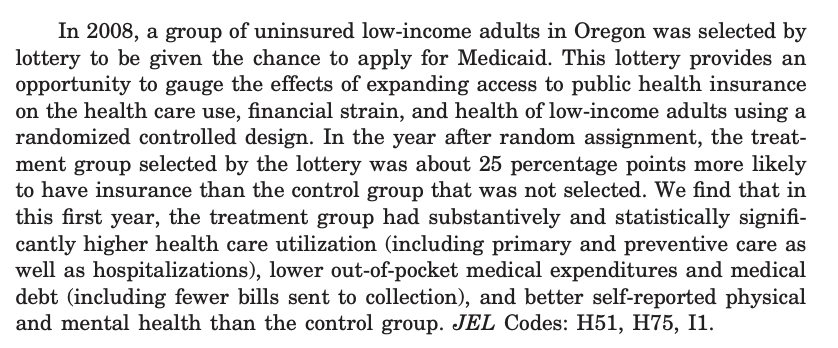
\includegraphics[width = 0.9\linewidth]{ohie-abstract}
	\end{frame}

	\begin{frame}{Winning the lottery vs Medicaid}
		\begin{wideitemize}
			\item
			Previously, we used the OHIE to estimate the causal effect of \textit{winning the eligibility lottery} \\
			
			\item
			But what if we actually care about the causal effect of \textit{enrolling in Medicaid}? 
			
			\pause
			\item
			Winning the lottery is not the same as enrolling in Medicaid: \medskip
			
			\begin{tabular}{lrr}
				& Treatment & Control \\ \hline
				Ever on Medicaid & 0.397 & 0.141
			\end{tabular}
			
			\pause
			\item
			Some people who win the lottery do not enroll (don't return form; no longer eligible)
			
			
			\item
			Some people who lose the lottery enroll anyway (become eligible by other criteria)
		\end{wideitemize}
	\end{frame}


	\begin{frame}{The effect of Medicaid enrollement on depression}
		
			\begin{tabular}{lrr}
			& Treatment & Control \\ \hline
			Ever on Medicaid & 0.397 & 0.141 \\
		   Depression symptoms & 0.306 &  0.329 
		   \end{tabular}
	
	
	\begin{wideitemize}
		\item
		What is the estimated effect of winning the lottery on Medicaid enrollment? \pause $0.397-0.141 = 0.256$
		
		\pause
		\item
		What is the estimated effect of winning the lottery on depression? \pause $0.306 - 0.329 = -0.023$
		
		\pause
		\item
		Say you want to estimate the effect of \textit{Medicaid enrollment} on depression? What would you do?
		
		\pause
		\item
		A natural estimate is to divide the effect on depression by the effect on enrollment: $-0.023 / 0.256 \approx -0.09$ $\rightarrow$ a 9 pp reduction per enrollee
		
		\pause
		\item
		This is called an \textbf{instrumental variables (IV)} estimate. When does it work? And how exactly do we interpret it?
	\end{wideitemize}
	
	\end{frame}


	\begin{frame}{Local Average Treatment Effects (LATE)}
	
	
	\begin{wideitemize}

		\item
		We will show that under certain assumptions, instrumental variables lets us identify a \textbf{local average treatment effect} (LATE).
		
		\pause
		\item
		This is the average treatment effect for \textbf{compliers}, i.e. people who are induced to take-up Medicaid by winning the lottery
		
		\pause
		\item
		This is a ``local'' effect in the sense that it doesn't tell us about the treatment effect for people whose Medicaid status is not affected by the experiment

		\pause
		\item
		Next, we'll go over the assumptions we need to identify the LATE with instrumental variables
	\end{wideitemize}
		
	\end{frame}

\begin{frame}{Four types of people}

We can divide the population into four types of people:
	
	\begin{wideitemize}
		\item
		\textbf{Always takers:} people who will enroll in Medicaid regardless of the outcome of the lottery
		
		\pause
		\item  \textbf{Never takers:} people who will never enroll in Medicaid regardless of the lottery
		
		\pause
		\item \textbf{Compliers:} people who enroll in Medicaid only if they win the lottery
		
		\pause
		\item \textbf{Defiers:} people who enroll in Medicaid only if they lose the lottery
			\begin{itemize}
				\pause
				\item 
				Defiers are weird, and often we will assume they don't exist (called \textit{monotonicity})
			\end{itemize}
	\end{wideitemize}

\end{frame}



\begin{frame}{Four types of people -- With Math}
	
		
	\begin{wideitemize}
		\item
		Let $D_i$ be an indicator for whether you are on Medicaid (treatment).\\
		Let $Z_i$ be an indicator for whether you won the lottery (\textit{instrument})
		
		\pause
		\item
		Introduce \text{potential treatments}, $D_i(1)$ and $D_i(0)$, analogous to the potential outcomes
			\begin{itemize}
				\item 
				$D_i(1)$ is treatment status if $Z_i=1$ (win the lottery)
				
				\item
				$D_i(0)$ is treatment status if $Z_i=0$ (lost the lottery)
				
			\end{itemize}
		

		\pause
		\item
		\textbf{Always takers:} people who will enroll in Medicaid regardless of the outcome of the lottery. \pause Always takers have $D_i(1) = D_i(0) = 1$
		
		\pause
		\item  \textbf{Never takers:} people who will never enroll in Medicaid regardless of the lottery. \pause Never takers have $D_i(1) = D_i(0) = 0$
			
		
		\pause
		\item \textbf{Compliers:} people who enroll in Medicaid only if they win the lottery. \pause Compliers have $D_i(1) = 1$ and $D_i(0) = 0$
		
		\pause
		\item \textbf{Defiers:} people who enroll in Medicaid only if they lose the lottery. \pause Defiers have $D_i(1) = 0$ and $D_i(0) = 1$
			
	\end{wideitemize}
	
\end{frame}



\begin{frame}{Key assumptions}
	\begin{wideitemize}
	\item
	\textbf{Independence:} The instrument (e.g. whether you win the lottery) is as good as randomly assigned, $Z_i \indep (Y_i(0),Y_i(1), D_i(0), D_i(1))$
	
	\pause
	\item
	\textbf{Relevance} Instrument affects the probability of treatment: $P(D_i = 1 | Z_i = 1) \neq P(D_i = 1 | Z_i = 0)$
		\begin{itemize}
			\item 
			This one is testable -- we saw that it does!
		\end{itemize}
	
	\item
	\textbf{Monotonicity:} No defiers: $D_i(1) \geq D_i(0)$ for all $i$
			\begin{itemize}
				\item 
				Seems reasonable that anyone who enrolls without winning would also enroll if they won
			\end{itemize}

	\end{wideitemize}	
\end{frame}


\begin{frame}{Final key assumption --- exclusion restriction!}
	
	\begin{wideitemize}
		\item
		The final key assumption, and often the most tenuous, is what's called the \textbf{exclusion restriction}
		
		\pause
		\item
		Intuitively, this says that the instrument $Z_i$ (whether you won the lottery) affects your outcomes \textit{only through the treatment} (whether you enrolled in Medicaid)
		
		\pause
		\item
		Mathematically, we have that $Y_i = D_i(Z_i) Y_i(1)  + (1- D_i(Z_i)) Y_i(0) $
		\medskip
			\begin{itemize}
				\item 
				Equivalently, can write the POs as $Y_i(d,z)$, then state the exclusion restriction as $Y_i(d,z) = Y_i(d)$. 
			\end{itemize}
		
		\pause
		\item
		This implies that the outcomes for the always-takers and never-takers doesn't depend on $Z_i$
	\end{wideitemize}
	
	
\end{frame}


\begin{frame}{Why might exclusion fail?}
	
\begin{wideitemize}
	\item
	Intuitively, exclusion fails if the instrument (e.g. winning the lottery) can affect your outcome even without changing your treatment sattus
	
	\pause
	\item
	Suppose in the OHIE that some always-takers would have had to wait longer to get on Medicaid if they hadn't won the lottery. Would that violate exclusion? 
	
	\pause
	\item
	Yes, if wait-time for Medicaid affects your health. 
	 
\end{wideitemize}	
\end{frame}



\begin{frame}{Graphical Illustration}
	
\only<1>{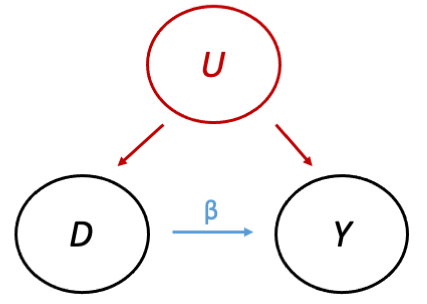
\includegraphics[width=0.5\linewidth]{dags/Slide2.png}}
\only<2->{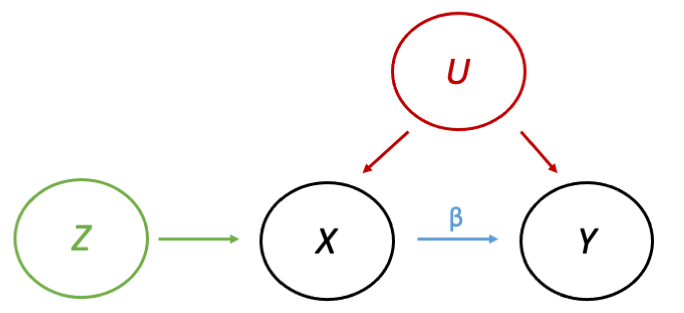
\includegraphics[width=0.5\linewidth]{dags/Slide3.png}}	
	
\begin{wideitemize}
	\item
	Unconfoundedness fails if there is an unobservable $U$ that affects both treatment $D$ and $Y$ (denoted by arrows)
	
	\pause
	\item
	We can get around this problem if we have instrument like $Z$
	
	\pause
	\item
	Independence: $Z$ is not influenced by the unobservable $U$ (it's randomly assigned!)
	
	\pause
	\item
	Exclusion: $Z$ affects $Y$ only through $D$ (no $Z \rightarrow Y$ arrow)
\end{wideitemize}	
\end{frame}


\begin{frame}{The LATE Theorem}

	\begin{wideitemize}
		\item
		If Independence, Relevance, Exclusion, and Monotonicity hold, then 
		
		$$ \dfrac{ \color{teal} E[Y_i | Z_i = 1] - E[Y_i | Z_i = 0 ]  }{  \color{blue} E[D_i | Z_i = 1] - E[D_i | Z_i = 0 ]   }  = {\color{red} E[Y_i(1) - Y_i(0) | D_i(1) = 1, D_i(0) = 0 ] } $$
		
		\noindent or in words:
		
		$$ \dfrac{ \color{teal} \text{Effect of $Z$ on $Y$}  }{  \color{blue} \text{Effect of $Z$ on $D$}   }  = {\color{red} \text{Local average treatment effect for compliers} } $$
		
		
		\pause
		\item
		This result won Joshua Angrist and Guido Imbens the 2021 Nobel Prize in Economics!
		
	\end{wideitemize}	
\end{frame}


\begin{frame}{Intuition for the LATE theorem}
\begin{wideitemize}
	\item
	Remember the theorem says that 
	
	$$ \dfrac{ \color{teal} E[Y_i | Z_i = 1] - E[Y_i | Z_i = 0 ]  }{  \color{blue} E[D_i | Z_i = 1] - E[D_i | Z_i = 0 ]   }  = {\color{red} E[Y_i(1) - Y_i(0) | D_i(1) = 1, D_i(0) = 0 ] } $$
	
	\pause
	\item
	By independence, the {\color{teal} numerator} is the causal effect of $Z$ on $Y$
	
	\pause
	\item
	However, the exclusion restriction says that the effect of $Z$ on $Y$ is zero for always-takers and never-takers (their treatment doesn't change!). \pause Further, we've assumed that there are no defiers
	
	\pause
	\item
	Thus,  the {\color{teal} numerator} will be the average effect for compliers times the fraction of compliers in the population, i.e. {\color{teal}  $LATE \times P(Complier)$ } 
	
	\pause
	\item
	But the {\color{blue} denominator} is the effect of $Z$ on $D$. This effect is zero for ATs and NTs, so the denominator is the share of compliers, ${\color{blue}  P(Complier)}$ 
	
\end{wideitemize}	
\end{frame}


\begin{frame}{More formal derivation}

\begin{wideitemize}
	\item
	Remember that we can divide the population into three groups, always-takers (ATs), never-takers (NTs), and compliers (Cs) \pause --- we assumed no defiers!
	
	\item
	Let $\alpha_{AT} = P(AT), \alpha_{NT} = P(NT), \alpha_{C} = P(C)$ be the shares of ATs, NTs, and Cs
	
	\pause
	\item
	Since $Z$ is randomly assigned (independence), we have that 
	$P(AT |  Z = 1) =\pause{} P(AT) = \alpha_{AT}$. \\ \pause
	Likewise, $P(AT |  Z = 0) =\pause{} P(AT) = \alpha_{AT}$
	
	\pause
	\item
	By similar arguments, share of NTs and Cs is the same in the $Z=1$ and $Z = 0$ groups.
\end{wideitemize}	
	
\end{frame}


\begin{frame}{More formal derivation}

\begin{wideitemize}
	
	\item
	Next step: show that the {\color{teal} numerator} is $\color{teal} \alpha_C \times LATE$
	
	\pause
	
	\item 
	By the Law of Iterated Expectations, 
	\begin{small}
	\begin{align*}
	 &E[Y_i | Z_i = 1]  = \pause{}\\ %
	&\alpha_C E[ Y_i | Z_i = 1, C ] +  \alpha_{AT} E[ Y_i | Z_i = 1, AT ] + \alpha_{NT}E[Y_i | Z_i  =1, NT] =\pause{}\\%
	& \alpha_C E[ Y_i(1) | Z_i = 1, C ] +  \alpha_{AT} E[ Y_i(1) | Z_i = 1, AT ] + \alpha_{NT}E[Y_i(0) | Z_i  =1, NT] = \pause{}\\
	& \alpha_C E[ Y_i(1) | C ] +  \alpha_{AT} E[ Y_i(1) | AT ] + \alpha_{NT}E[Y_i(0) |  NT]
	\end{align*} 
	\end{small}	
	\noindent where the last line uses independence
	\item
	Similarly,
		\begin{small}
		\begin{align*}
			&E[Y_i | Z_i = 0]  = \pause{} \alpha_C E[ Y_i(0) | C ] +  \alpha_{AT} E[ Y_i(1) | AT ] + \alpha_{NT}E[Y_i(0) |  NT] %
		\end{align*} 
	\end{small}	

	\item
	Thus, the numerator in our ratio is 
	$$ \color{teal} E[Y_i | Z_i = 1] - E[Y_i | Z_i = 0]  = \alpha_C \underbrace{(E[Y_i(1) | C]  - E[Y_i(0) | C])}_{LATE}$$  
\end{wideitemize}	
	
\end{frame}


\begin{frame}{More formal derivation}

\begin{wideitemize}
	\item
	We showed that the {\color{teal} numerator} is $\color{teal} \alpha_C \times LATE$
	
	\item
	To finish proof, we show that the $\color{blue} denominator$ is $\color{blue} \alpha_C$
	
	\pause
	\item
	The denominator is 
	
	\begin{align*}
		\color{blue} E[D_i | Z_i = 1] - E[D_i | Z_i = 0] &= \pause{}  \color{blue} Pr(\text{AT or C} | Z_i = 1) - P(\text{AT} | Z_i = 0)  \pause{} \\
		& = \color{blue}  (\alpha_C + \alpha_{AT}) - \alpha_{AT} = \pause{}  \color{blue}  \alpha_C
	\end{align*} 


	\pause
	Hence, $$\dfrac{\color{teal} numerator}{ \color{blue}  denominator }	= \dfrac{\color{teal} \alpha_C \times LATE}{ \color{blue}  \alpha_C } = \color{red} LATE$$
\end{wideitemize}	
	
\end{frame}


\begin{frame}{Estimating LATE}
	
	\begin{wideitemize}
		\item
		We've shown that under the IV assumptions, the LATE is identified as a function of population means
		
		$$ \dfrac{ \color{teal} E[Y_i | Z_i = 1] - E[Y_i | Z_i = 0 ]  }{  \color{blue} E[D_i | Z_i = 1] - E[D_i | Z_i = 0 ]   }  = {\color{red} \text{LATE}} $$
		
		
		\item
		How can we estimate LATE? 
		
		\pause
		\item
		Plug in sample means!
		
		$$\hat\beta =  \dfrac{  \bar{Y}_{Z=1} - \bar{Y}_{Z=0}   }{ \bar{D}_{Z=1} - \bar{D}_{Z=0} } , $$
		
		\noindent where, e.g., $\bar{Y}_{Z=1}$ is the sample mean of $Y_i$ for units with $Z_i = 1$
		
		
		\pause
		\item
		$\hat\beta$ is called the IV estimator, or more precisely, the two-stage least squares (2SLS) estimator (for reasons that will become clear soon!)
	\end{wideitemize}
\end{frame}


\begin{frame}{Example - Medicaid}
			\begin{tabular}{lrr}
	& Treatment & Control \\ \hline
	Ever on Medicaid & 0.397 & 0.141 \\
	Depression symptoms & 0.306 &  0.329 
\end{tabular}

\bigskip 
\begin{wideitemize}
	\item
	Let's calculate the 2SLS estimator in the Medicaid example.
	
	\pause
	$$ \dfrac{  \bar{Y}_{Z=1} - \bar{Y}_{Z=0}   }{ \bar{D}_{Z=1} - \bar{D}_{Z=0} }  = \pause{} \frac{0.306 - 0.329}{0.397 - 0.141}  = \pause{} -0.09$$
	
\end{wideitemize}


\end{frame}



\begin{frame}{Two-stage least squares}

\begin{wideitemize}
	\item
	Consider the two linear regressions:
	\begin{align}
		&Y_{i} = \gamma_0 +   Z_i \gamma_1 + \epsilon_{i} \\
		&D_i = \pi_0 + Z_i \pi_1 + u_i
	\end{align}

	\item
	What are the OLS estimates $\hat\gamma_1$ and $\hat\pi_1$? 
	
	\pause
	\begin{align*}
		\hat\gamma_1 = \bar{Y}_{Z=1} - \bar{Y}_{Z=0} \\ \pause{}
		\hat\pi_1 = \bar{D}_{Z=1} - \bar{D}_{Z=0}
	\end{align*}

	
	\pause
	\item
	Thus, the 2SLS estimator is the ratio of these two OLS coefficients:
	
	$$\hat\beta =  \dfrac{  \bar{Y}_{Z=1} - \bar{Y}_{Z=0}   }{ \bar{D}_{Z=1} - \bar{D}_{Z=0} } = \frac{\hat\gamma_1}{\hat\pi_1} $$
	
	
	\pause
	\item
	Equation (2) is typically called the \textit{first-stage}, while equation (1) is called the \textit{reduced form}
\end{wideitemize}	
	
\end{frame}


\begin{frame}{Example - Medicaid}
	\begin{tabular}{lrr}
		& Treatment & Control \\ \hline
		Ever on Medicaid & 0.397 & 0.141 \\
		Depression symptoms & 0.306 &  0.329 
	\end{tabular}
	
	\bigskip 
	\begin{wideitemize}
		\item
		What is the ``first-stage'' coefficient from 
		$$D_i = \pi_0 + Z_i \pi_1 + u_i?$$
		
		\pause
		\item
		$\hat\pi_1 = 0.397 - 0.141 = 0.256$
		
		\pause
		\item
		What is the ``reduced-form'' coefficient from 
		$$Y_i = \gamma_0 + Z_i \gamma_1 + \epsilon_i?$$
		
		\pause
		\item
		$\hat\gamma_1 = 0.306 - 0.329 = -0.023$
		
		\pause
		\item
		So the 2SLS estimator is $\hat\gamma_1/\hat\pi_1 = -0.023/0.256 = -0.09$.
	\end{wideitemize}
	
\end{frame}


\begin{frame}{IV conditional on covariates}
	\begin{wideitemize}
		\item
		Oftentimes, the assumption that the instrument is as-good-as-randomly assigned will only be plausible conditional on observable characteristics
		
		\item
		In fact, in the OHIE, the probability of winning the lottery depended on family size!
		
		\pause
		\item
		Suppose that we replace the independence assumption with conditional independence, $Z_i \indep (Y_i(1),Y_i(0),D_i(1), D_i(0)) | X_i$
		
		\item
		By similar arguments as before, we can identify the \textit{conditional LATE} by taking the same ratio within groups with the same value of $x$
		
		\begin{align*}
			&\dfrac{ \color{teal} E[Y_i | Z_i = 1, X_i = x] - E[Y_i | Z_i = 0, X_i = x ]  }{  \color{blue} E[D_i | Z_i = 1, X_i = x] - E[D_i | Z_i = 0 , X_i = x]   }  = \\&{ \color{red}  \underbrace{ E[Y_i(1) - Y_i(0) | D_i(1) = 1, D_i(0) = 0, X_i = x] }_{\text{LATE(x)}} }
		\end{align*}
		
		
	\end{wideitemize}	
\end{frame}


\begin{frame}{Estimation for LATEs conditional on covariates}

\begin{wideitemize}
	\item
	In practice, when we have conditional independence for the instrument, people estimate a modified version of 2SLS that includes covariates.
	
	\item
	That is, they use $\hat\beta_{2SLS} = \hat\gamma_1 / \hat\pi_1$, for the OLS estimates from
	
		\begin{align}
		&Y_{i} = \gamma_0 +   Z_i \gamma_1 + \bm{X}_i' \bm{\gamma}_2 + \epsilon_{i} \label{eqn: rf w covariates}\\
		&D_i = \pi_0 + Z_i \pi_1 + \bm{X}_i'\pi_2 +  u_i \label{eqn: fs w covariates}
	\end{align}
	
	\pause 
	
	\item
	When $\bm{X}_i$ is a set of dummy variables for different categories (e.g. family size), this gives a weighted average of the 2SLS estimates for each covariate value
	
	\pause
	\item
	More generally, this will be approximately consistent for a weighted average of $LATE(x)$ when (\ref{eqn: fs w covariates}) is a good approximation to the CEF
	
\end{wideitemize}

\end{frame}


\begin{frame}{Example - Medicaid}
	\begin{wideitemize}
		\item
		In the OHIE, the lottery was actually only random condition on family size
		
		\pause
		\item
		Finkelstein et al (2012) therefore estimate 2SLS with 
		
			\begin{align}
			&Y_{i} = \gamma_0 +   Z_i \gamma_1 + \bm{X}_i' \bm{\gamma}_2 + \epsilon_{i} \\
			&D_i = \pi_0 + Z_i \pi_1 + \bm{X}_i'\pi_2 +  u_i 
		\end{align}
		
		\noindent where $\bm{X}_i$ includes fixed effects for family size and some other demographic variables. 
					
	\end{wideitemize}
\end{frame}


\begin{frame}
	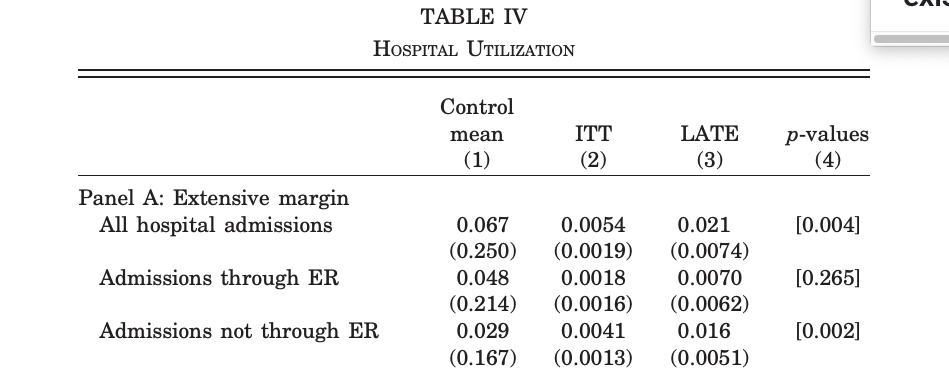
\includegraphics[width = 0.9\linewidth]{finkelstein-results-er}
\end{frame}


\begin{frame}
	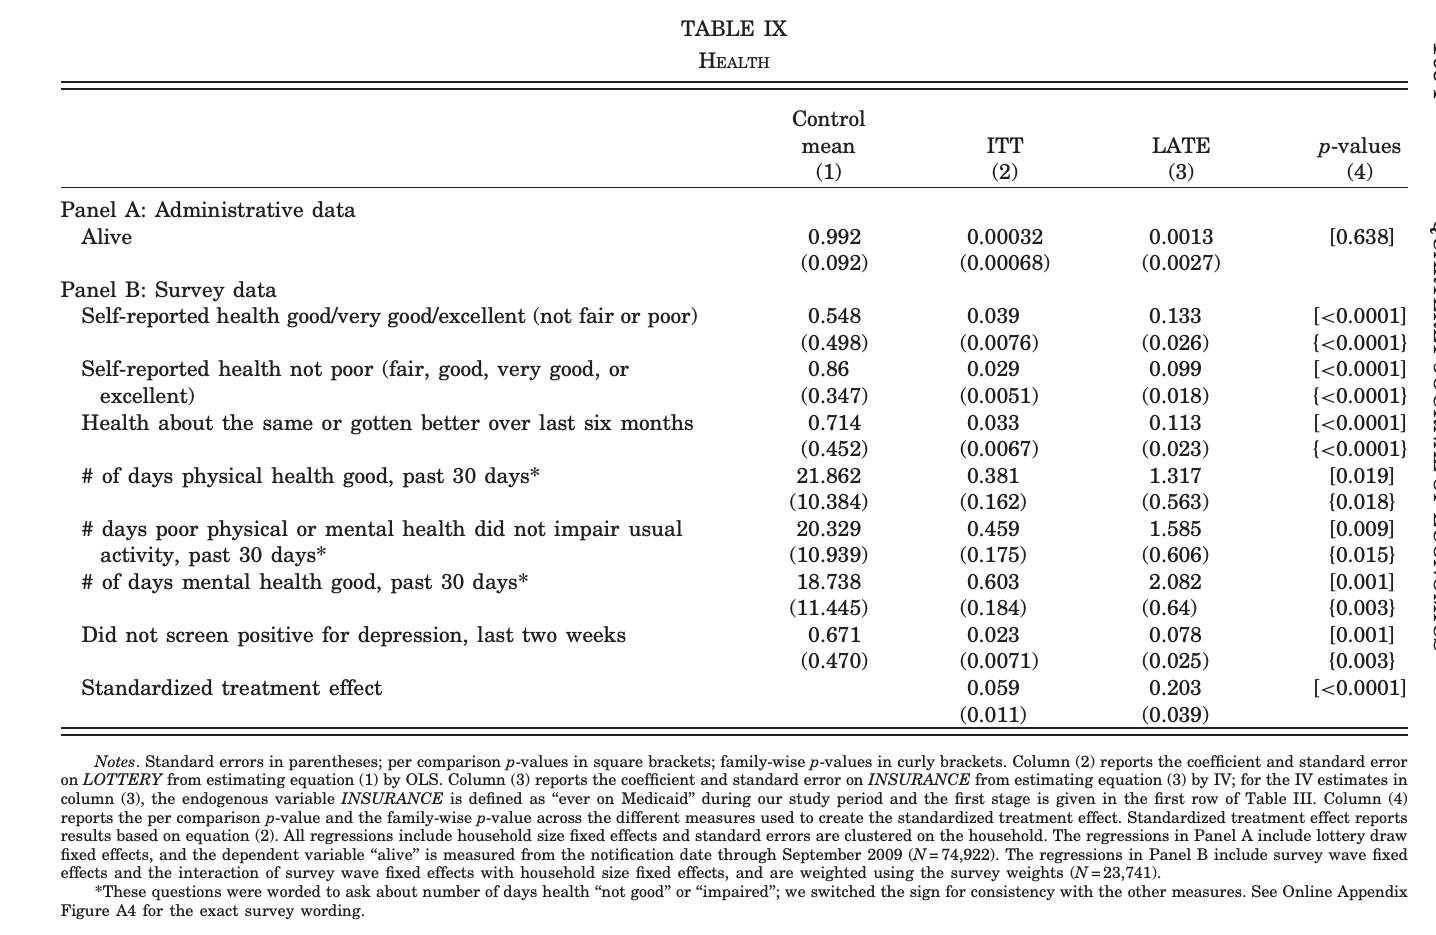
\includegraphics[width = 0.9\linewidth]{finkelstein-results-depression}
\end{frame}


\begin{frame}{``Quasi-experimental'' Instruments}
	
	\begin{wideitemize}
		\item
		In the Oregon Medicaid setting, the instrument $Z_i$ was explicitly randomly assigned
		
		\pause
		\item
		In other settings, researchers use an instrument that is not directly randomly but may be the result of idiosyncratic factors that are potentially ``as good as random''
		
		\item
		This expands the set of cases where we can use IV, but means the required assumptions deserve extra scrutiny! 
	\end{wideitemize}
	%%XX explain exogeneity? 
\end{frame}


\begin{frame}{Example -- Angrist and Krueger (1991)}
	\begin{wideitemize}
		\item
		AK (1991) are interested in a classic question in labor economics: what are the labor market returns to an additional year of schooling? 
		
		\pause
		\item
		Why can't we just compare earnings for people who get more or less schooling? 
			\pause
			\begin{itemize}
				\item 
				Schooling is not randomly assigned! Choice of schooling may depend on many confounding factors, such as ability or family background, that would directly affect earnings as well. 
			\end{itemize}
		
		\pause
		\item
		What do we need if we want to estimate the effects of schooling on earnings using IV? 
		
		\pause
		\item
		We need to find an instrument that is as-good-as-randomly assigned, and affects earnings only through years of schooling.  
	\end{wideitemize}
\end{frame}


\begin{frame}{Compulsory Schooling Laws}
	\begin{wideitemize}
		\item
		Most states have compulsory schooling laws that require people to stay in school until their 16th or 17th birthday
		
		\pause
		\item
		AK argue that these laws will lead people planning to drop out to have less schooling if they are born earlier in the year
		
		\item
		That is, if the oldest kid in a class is born on January 1 and the youngest kid is born on December 31, then the oldest kid can legally drop out after getting 1 fewer year of education than the youngest kid
		
		
		\pause
		\item
		AK argue that the part of the year in which you are born is effectively random, and therefore instrument for years of schooling with quarter of birth
	\end{wideitemize}
\end{frame}


\begin{frame}{}
	\centering
	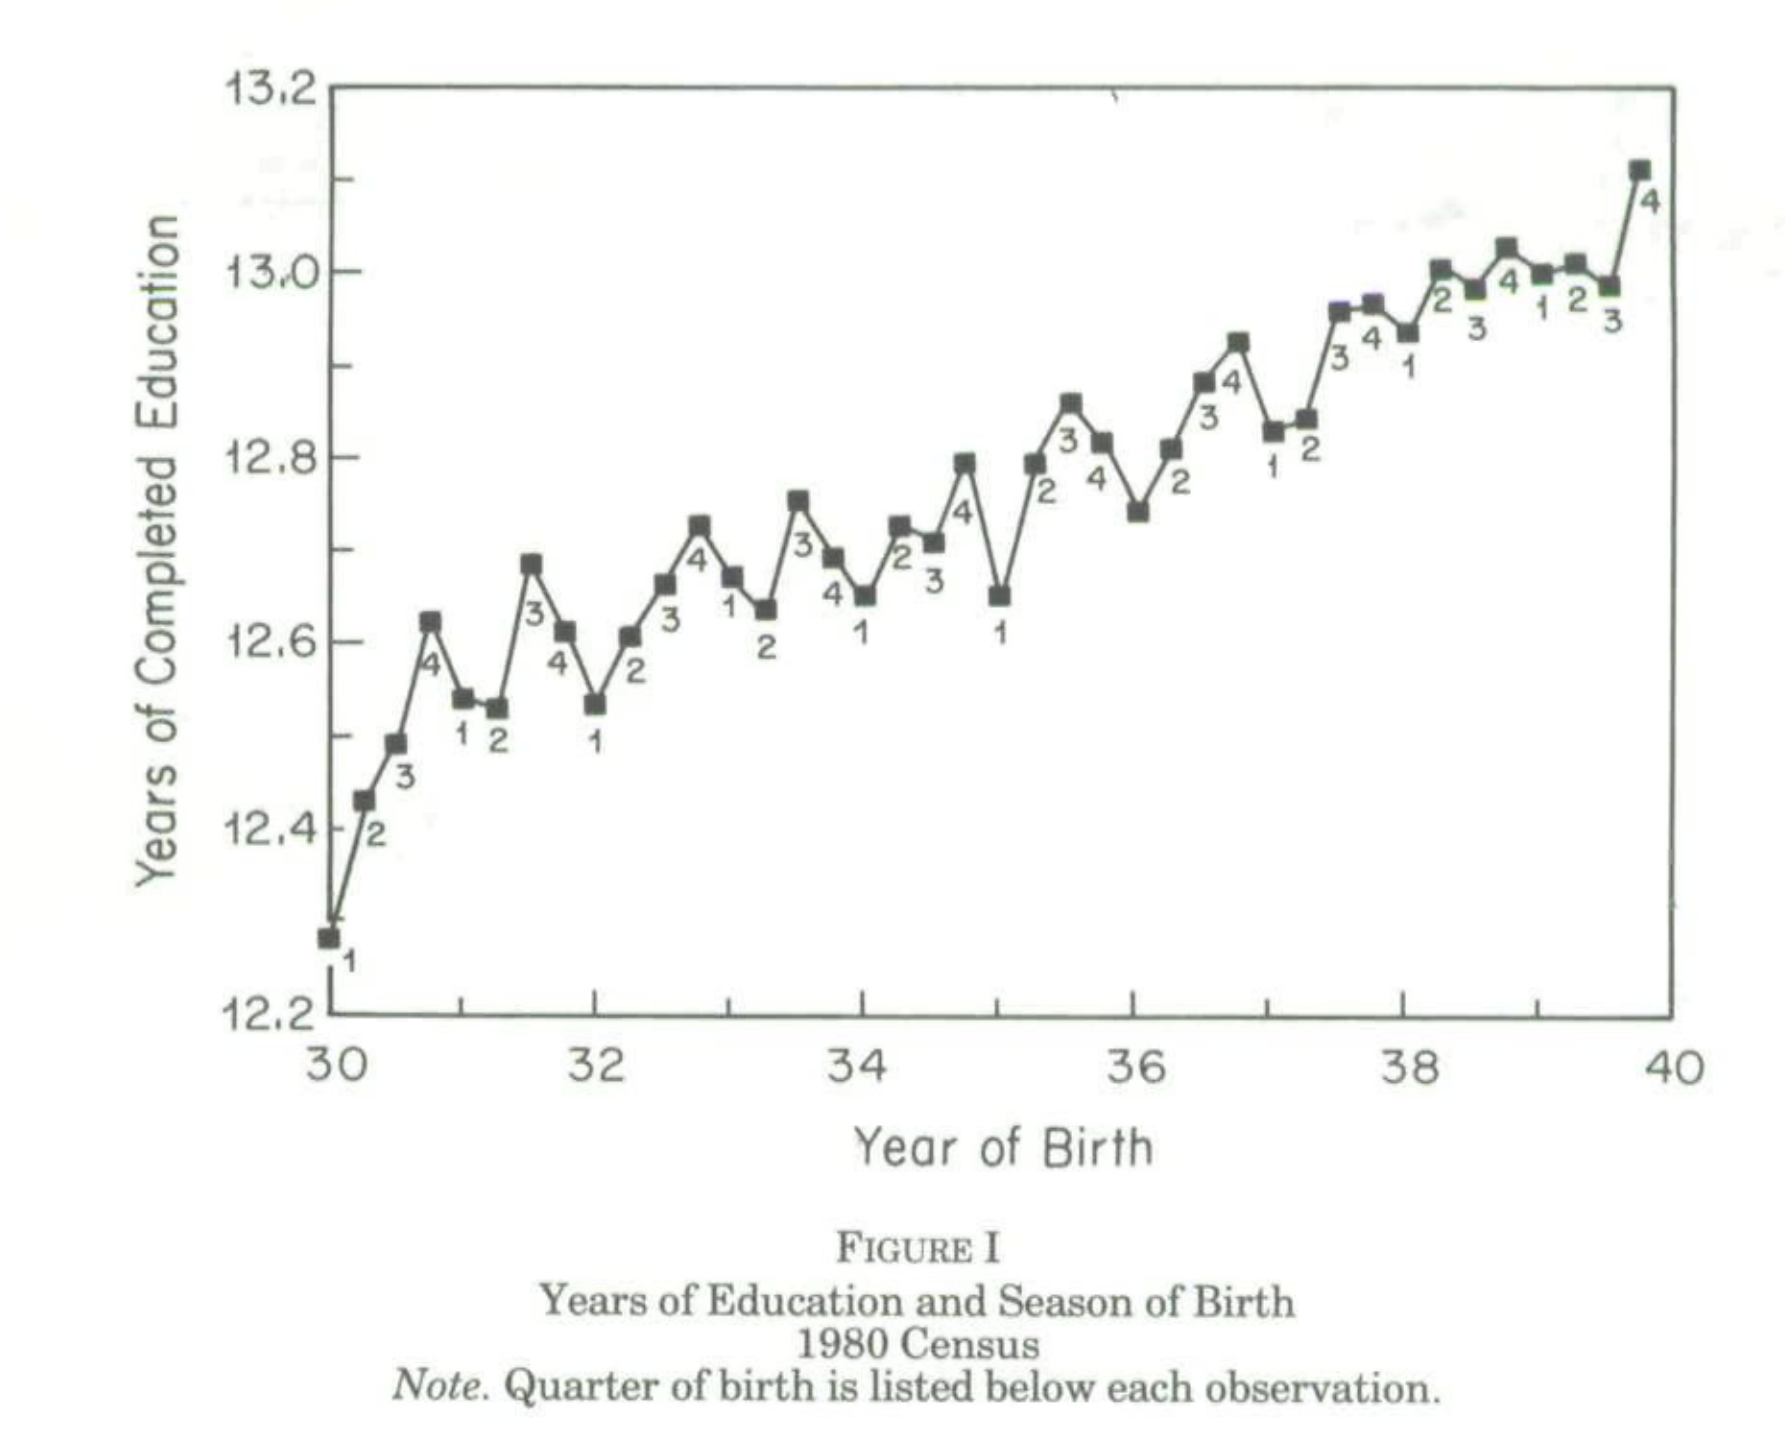
\includegraphics[width = 0.7 \linewidth]{ak-first-stage-graph}
	
	\begin{wideitemize}
		\item
		Indeed, AK find that people born in the first quarter the of the year tend to have less schooling on average than people born in the remaining three quarters of the same year
	\end{wideitemize}
\end{frame}

\begin{frame}
	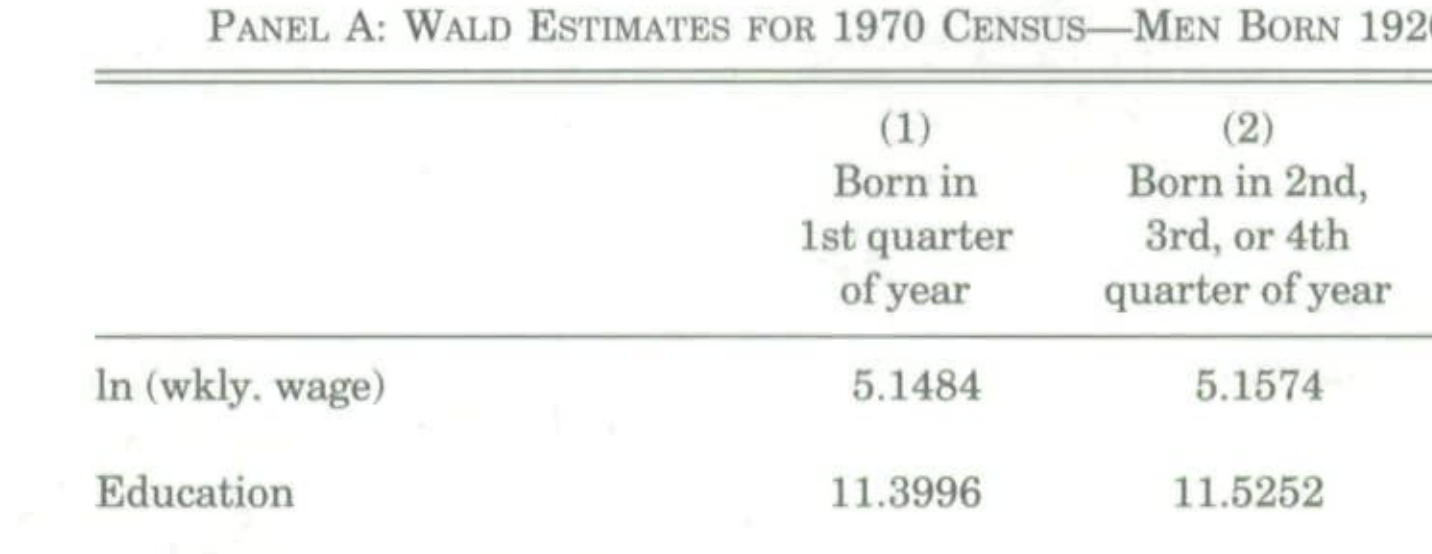
\includegraphics[width = 0.7 \linewidth]{ak-first-stage-basic}
	
	\pause
	\begin{wideitemize}
		\item
		What is the first stage estimate? \pause{} $11.5252 - 11.3996 = 0.1256$
		
		\pause
		\item
		What is the reduced form estimate? \pause{} $5.1574 - 5.1484 = 0.0090$
		
		\pause
		\item
		What is the 2SLS estimate? \pause{} $0.0090 / 0.1256 = 0.0715$
	\end{wideitemize}
\end{frame}


\begin{frame}
		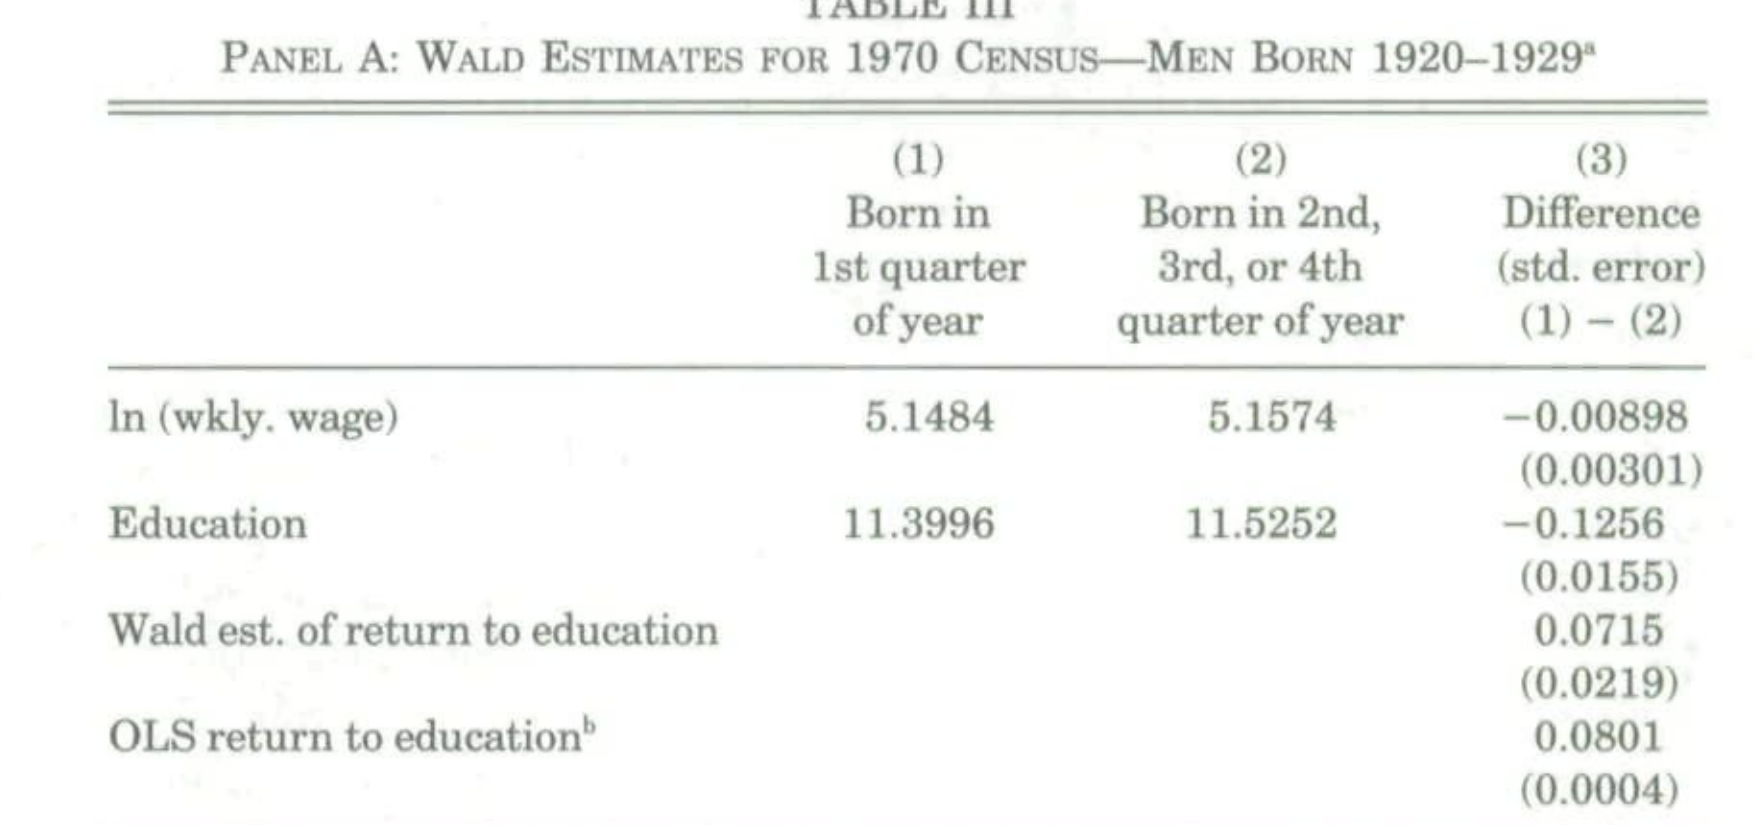
\includegraphics[width = 0.9 \linewidth]{ak-first-stage}
\end{frame}


\begin{frame}{Evaluating the assumptions}
	\begin{wideitemize}
		
		\item \textbf{Relevance:} \pause{} Need quarter of birth to be correlated with years of education. \pause{} \\
		$\checkmark$ This one we can check and indeed is the case ($t$-statistic of 12).
		
		
		\pause
		\item \textbf{Independence:} \pause Need quarter of birth to be independent of determinants of wages or responses to compulsory schooling laws ($Z_i \indep (Y(.), D(.)))$). 
		
		\pause
		\item
		Independence seems plausible if parents can't time the births of their children exactly. \pause{} But...
	\end{wideitemize}	
	
\end{frame}

\begin{frame}
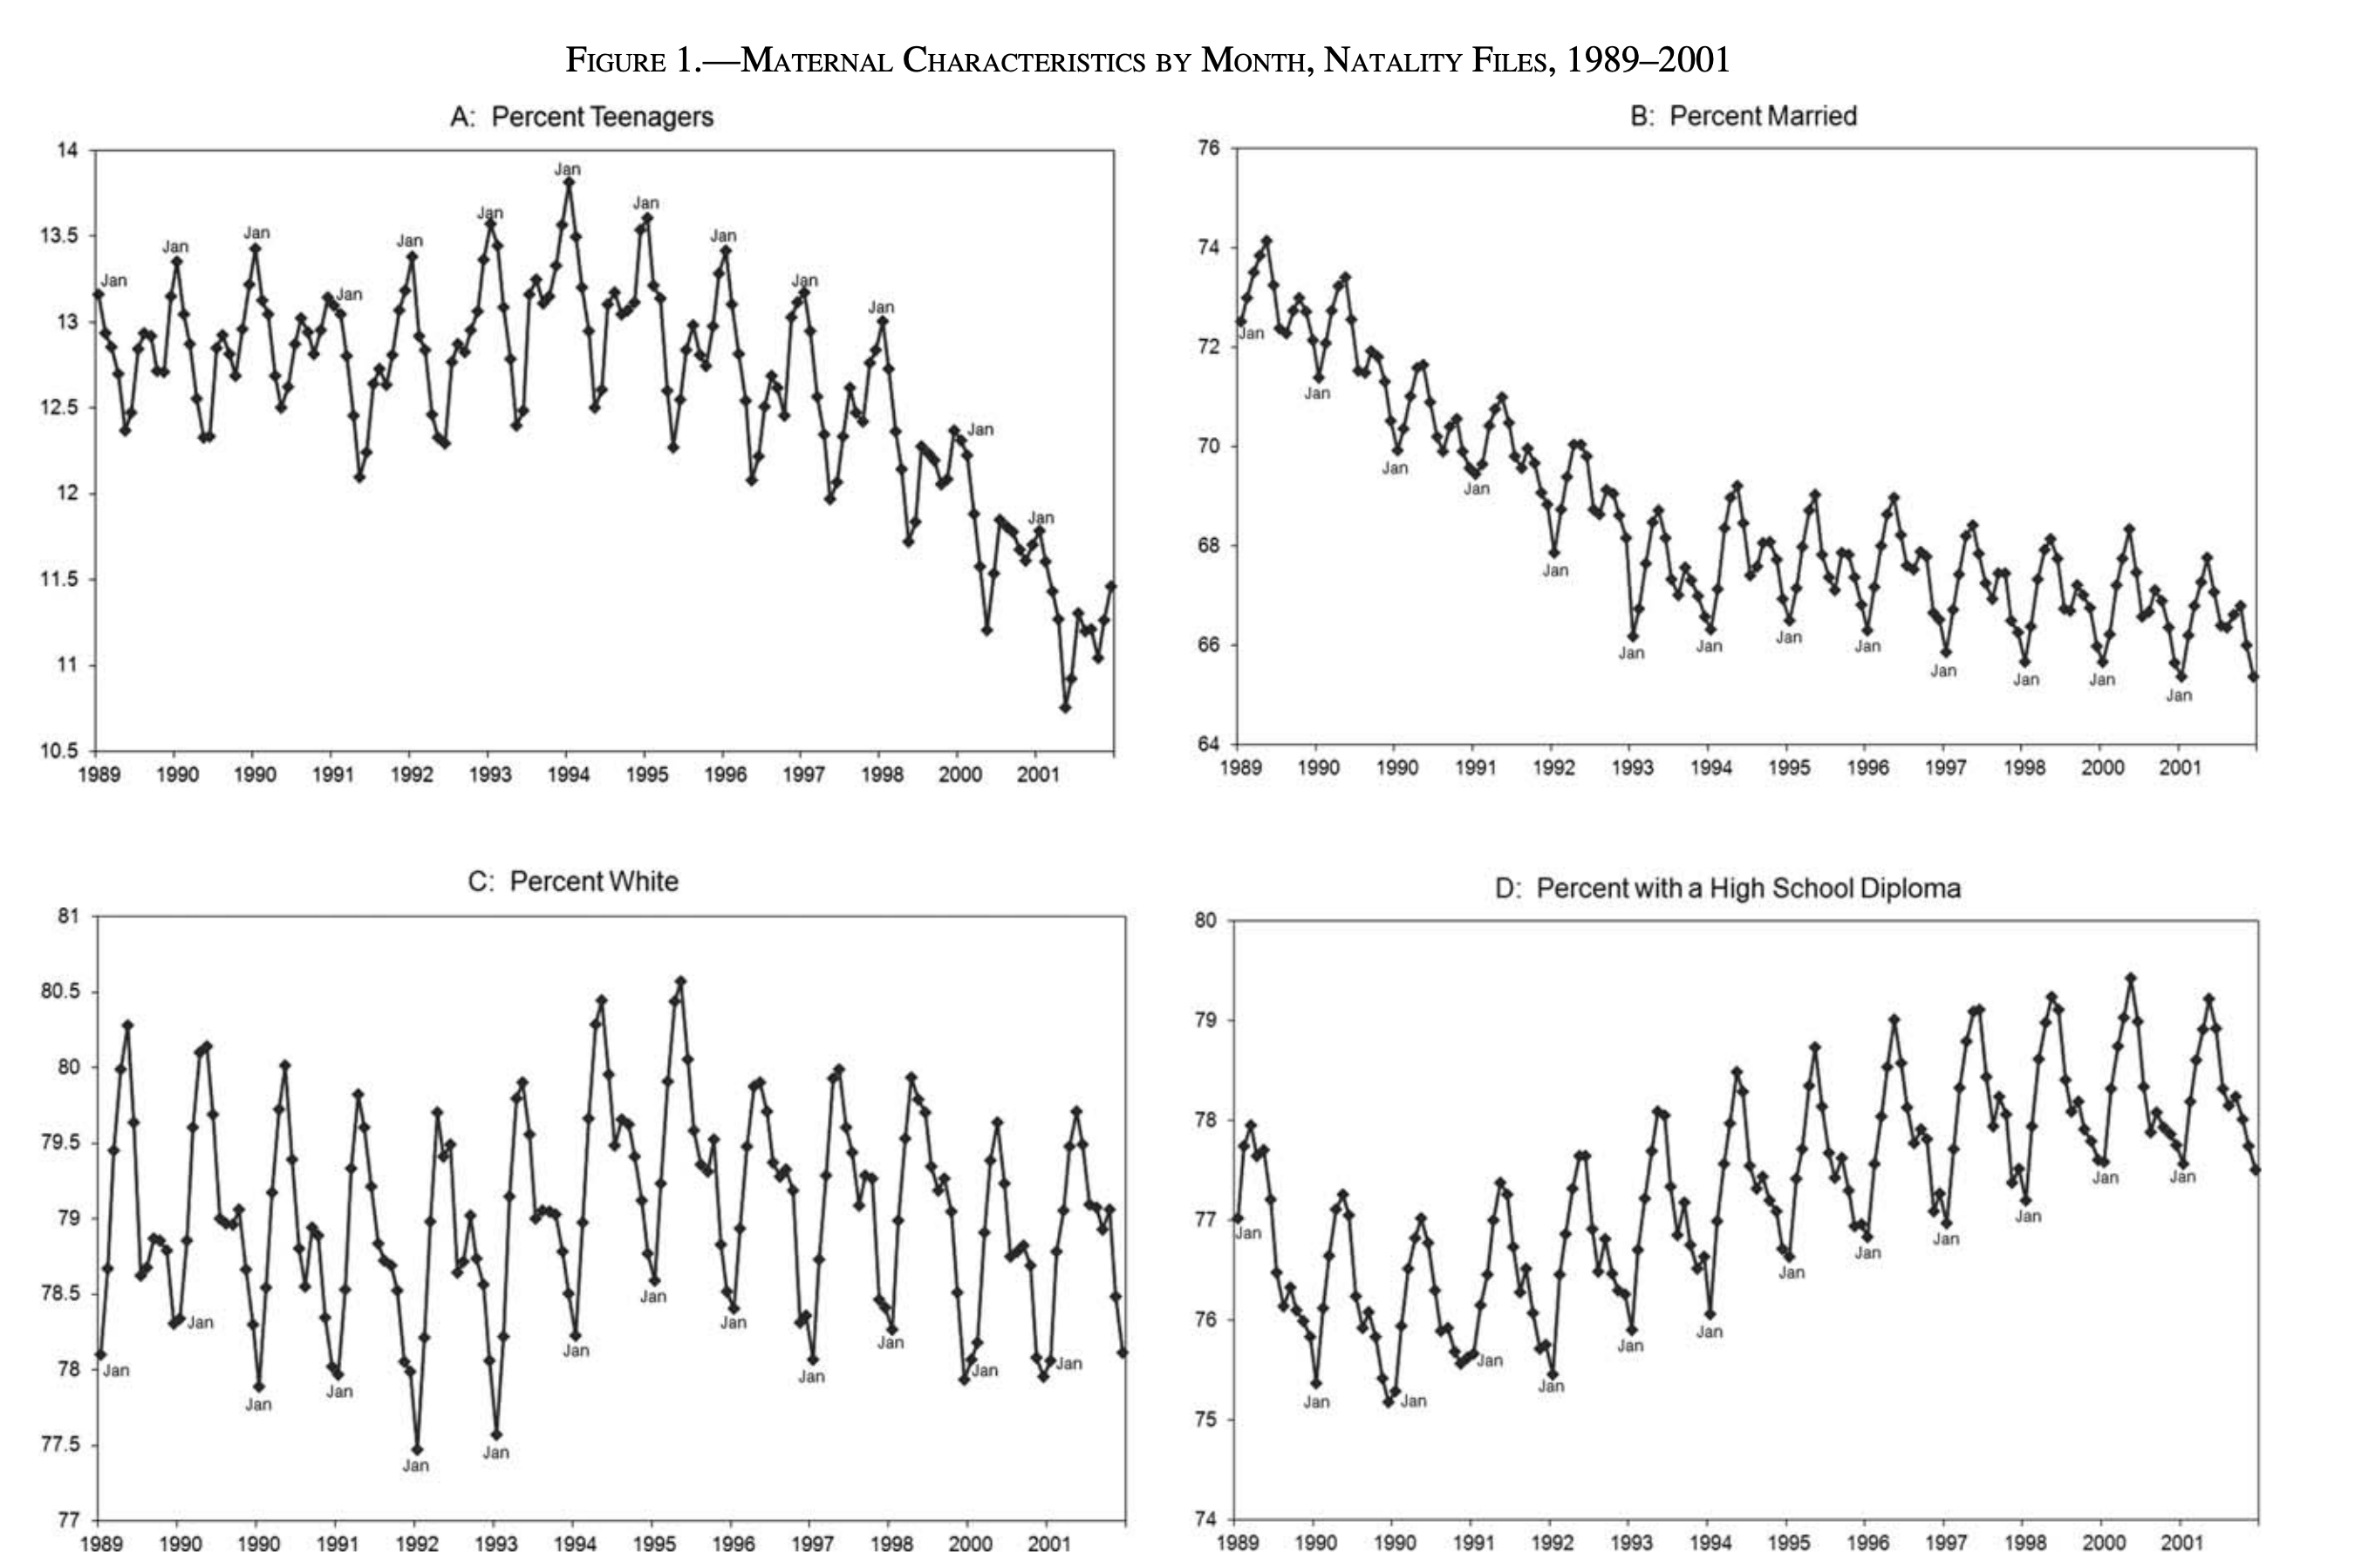
\includegraphics[width = 0.8\linewidth]{qob-characteristics}

\begin{wideitemize}
	\item
	Quarter of birth is correlated with some demographic characteristics
	
	\item
	Suggests some possible violations of independence
\end{wideitemize}
\end{frame}


\begin{frame}{Evaluating the assumptions...}
	
	\begin{wideitemize}
		\item
		\textbf{Exclusion: } Quarter of birth affects earnings only through number of years of education
		
		\pause
		\item
		Implies that people whose years of schooling are unaffected by QOB would have same wages if born at different time of the year
		
		\pause
		\item 
		Seems generally plausible but... \pause{} being older or younger in your grade may affect the quality of your education directly
					
	\end{wideitemize}
\end{frame}


\begin{frame}
	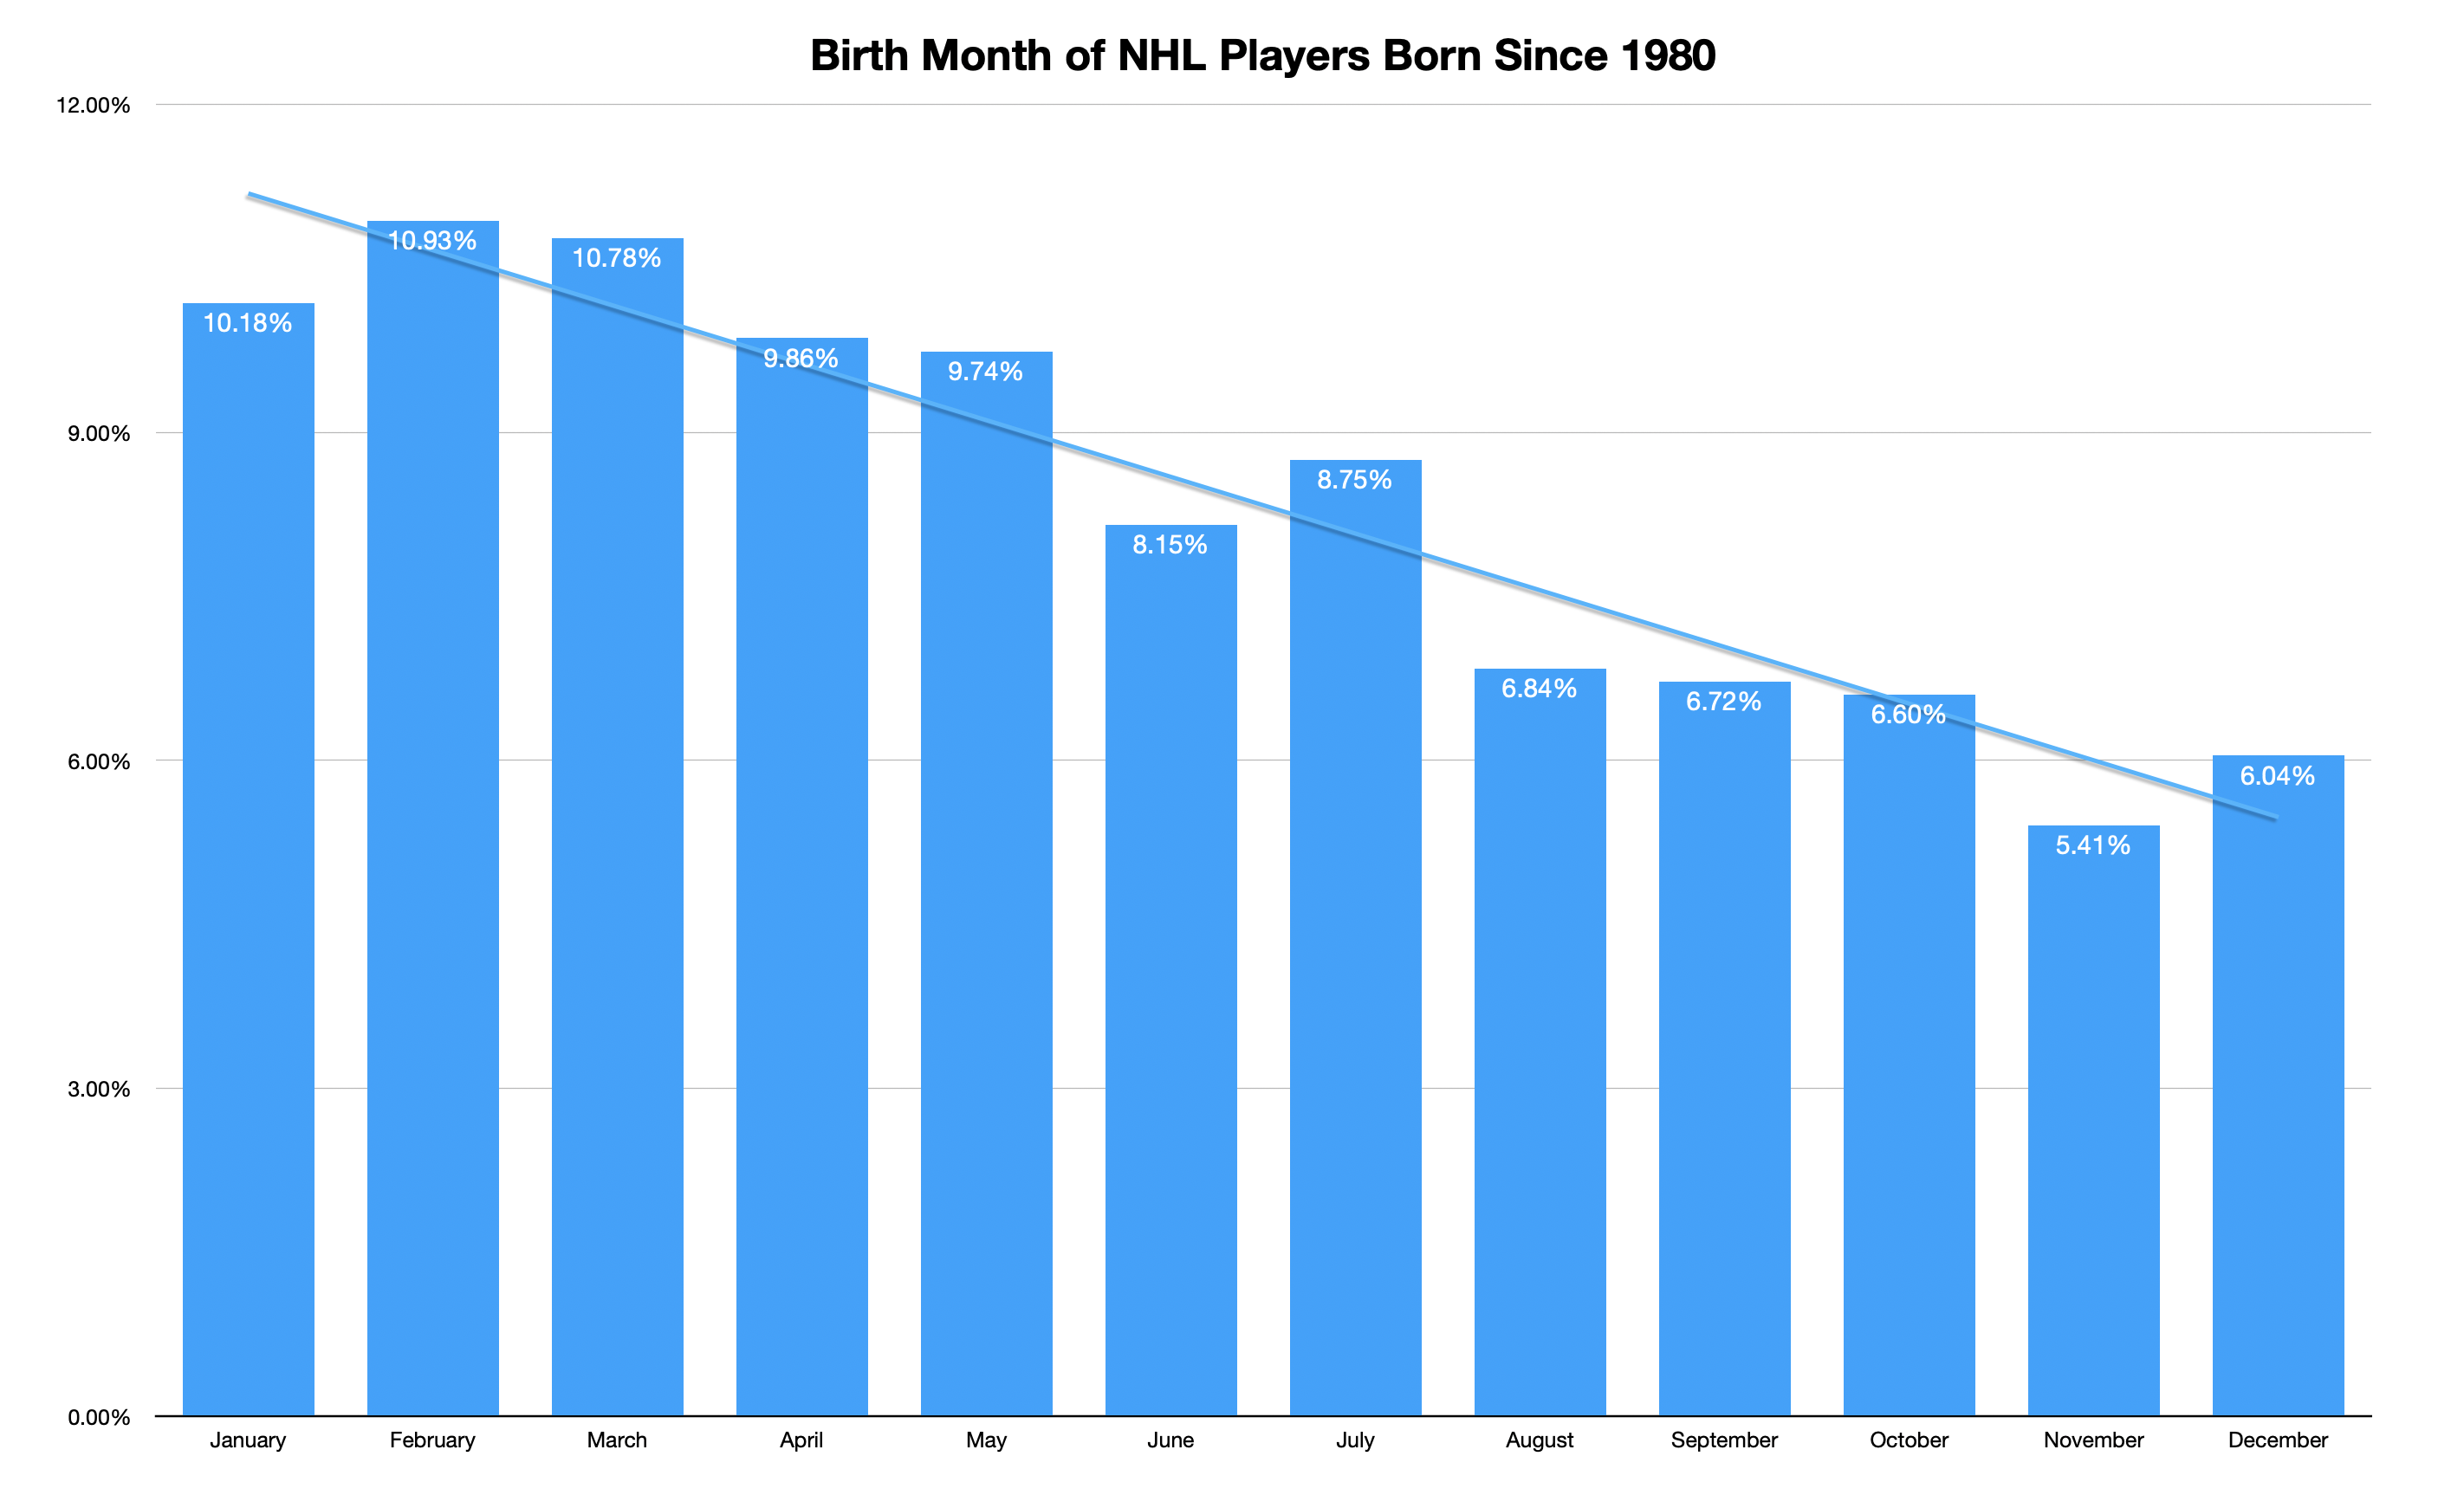
\includegraphics[width = 0.7\linewidth]{nhl-births}
\end{frame}

\begin{frame}
	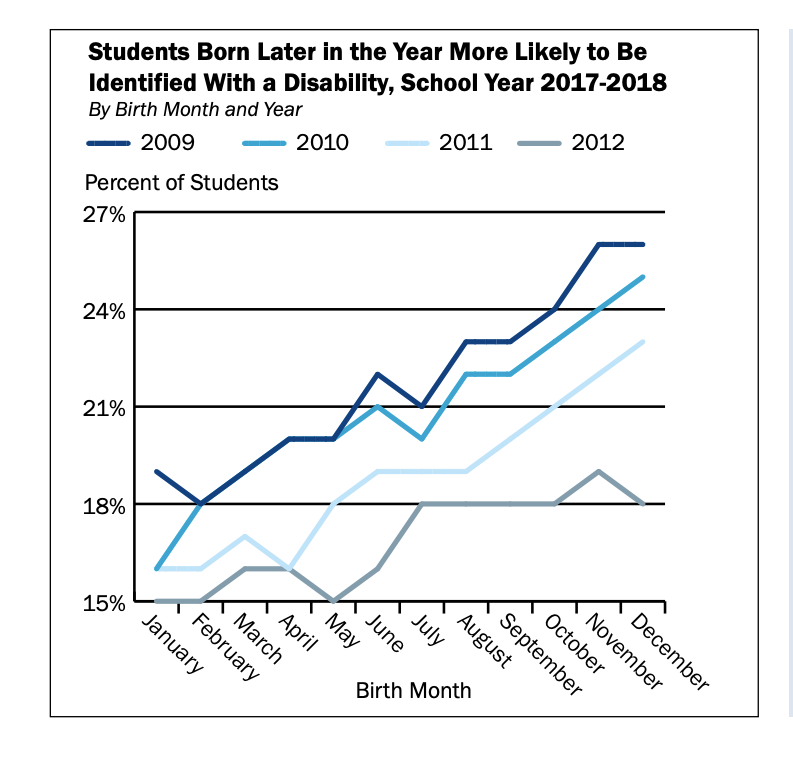
\includegraphics[width = 0.7 \linewidth]{qob-disabilities}
\end{frame}

\begin{frame}{Evaluating the assumptions}
	\begin{wideitemize}
		\item
		\textbf{Monotonicity:} Everyone would get at least as many years of schooling if not born in the first quarter of the year
		
		\pause
		\item
		Seems reasonable if all schools use a January 1 cutoff for school grades
		
		\pause
		\item
		If some schools use a Sept 1 cutoff, it could be that being born in Q4 is even worse
	\end{wideitemize}
\end{frame}


\begin{frame}
	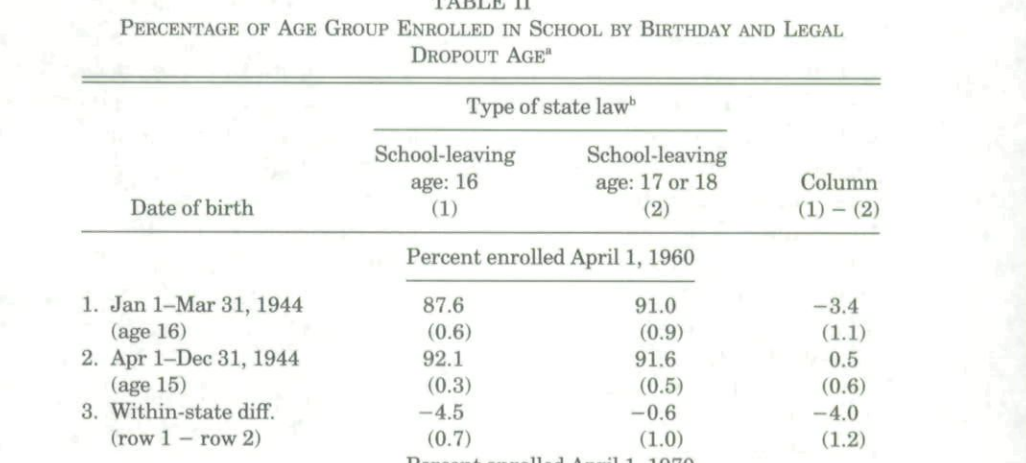
\includegraphics[width = 0.7 \linewidth]{qob-placebo}
	
	\bigskip
	
	\pause
	\begin{wideitemize}
		\item
		Comparing states with different-aged CSLs suggested the effects of QOB on education operates through the CSL $\rightarrow$ assuages some of (but not all) concerns about independence
	\end{wideitemize}
\end{frame}

\begin{frame}{A treatment effect for whom?}
	\begin{wideitemize}
		\item
		Suppose that we believe the IV assumptions hold (approximately).
		
		\item
		How do we interpret the treatment effect we estimate? 
		
		\pause
		\item
		It is a Local Average Treatment Effect (LATE) for compliers --- i.e. people who would have gotten an extra year of school if they'd been born in the latter part of the year
		
		\pause
		\item
		Why might the LATE not correspond with the ATE for the whole population? 
		
			\pause
			\begin{wideitemize}
				\item
				Treatment effects could be different for people on the margin of dropping out
			\end{wideitemize}
	\end{wideitemize}
	
\end{frame}


\begin{frame}{Multiple Instruments}
	\begin{wideitemize}
		\item
		So far, we have considered binary instrumental variables (win vs lose lottery)
		
		\item
		Sometimes we may have an instrument that takes on multiple values (or multiple different instruments) 
		
		
		\item
		Next we'll talk about how we can use similar ideas to exploit the variation from multi-valued instruments
				
	\end{wideitemize}
\end{frame}

\begin{frame}{Example -- Angrist 1990}
	\begin{wideitemize}
		\item
		Angrist (1990) is interested in the following Q: how does serving in the military (particularly the Vietnam War) affect your labor market earnings later in life? 
		
		\pause
		\item
		Why can't we we just compare veterans to non-veterans?
			\pause
			\begin{itemize}
				\item 
				Veteran status is non-random! Veterans may differ in career goals, family background, physical ability, etc. 
			\end{itemize}
		
		\pause
		\item
		If we want to use IV, what do we need? \pause A plausibly random instrument that affects earnings only through whether you enroll in the military
	\end{wideitemize}
\end{frame}

\begin{frame}{Angrist 1990 -- Draft Lotteries}
	\begin{wideitemize}
		\item
		Angrist (1990) exploits the fact that during the Vietnam War there was a compulsory draft (for men)
		
		\item
		In the 1970s, the military conducted lotteries where each birthday was randomly assigned a priority number. People born on a birthday with a lower number were eligible to be drafted first
		
		\pause
		\item
		Lottery numbers did not entirely determine whether one served in the military or not:
		
			\begin{itemize}
				\item 
				Some people with low numbers were given medical exemptions or left the country
				
				\item
				Some people with high numbers volunteered to serve in the military anyway
			\end{itemize} 
		
		\pause
		\item
		Angrist first considers a binary version of the instrument (eligible vs non-eligible bdays), then generalizes to multiple instruments (one for each bday)
	\end{wideitemize}
\end{frame}


\begin{frame}{Evaluating the IV assumptions}
	\begin{wideitemize}
		\item
		\textbf{Independence:} \pause{} Need lottery numbers to not be systematically related to potential earnings / potential enrollment \pause
			\begin{itemize}
				\item 
				Randomization of the lottery makes this plausible
				\item
				People with high/low numbers are similar on observable characteristics
			\end{itemize}
		
		\item
		\textbf{Exclusion:} \pause{} Need lottery number to affect earnings only through enrollment
			\pause
			\begin{itemize}
				\item 
				Exclusion in this context is a bit tricky
				
				\item
				Never-takers might have to flee the country if they have a low number but not a high one
				
				\item
				Always-takers might have a different army experience if they enroll voluntarily
			\end{itemize}
		
		
		\item
		\textbf{Relevance:} \pause{} Lottery numbers must affect whether someone enrolls \pause 
			\begin{itemize}
				\item 
				Reasonable -- and we'll see it's true!
			\end{itemize}
		
		\pause
		\item
		\textbf{Monotonicity:} Everyone who would enroll with a high number would also enroll with a low number \pause
			\begin{itemize}
				\item Seems reasonable
			\end{itemize}
		
	\end{wideitemize}
\end{frame}


\begin{frame}
	\begin{wideitemize}
		\item
		Angrist first considers a binarized version of the instrument where he groups birthdays into eligible and non-eligible
		
		\item
		Here is his first stage (see $\hat{p}^e - \hat{p}^n$)
	\end{wideitemize}
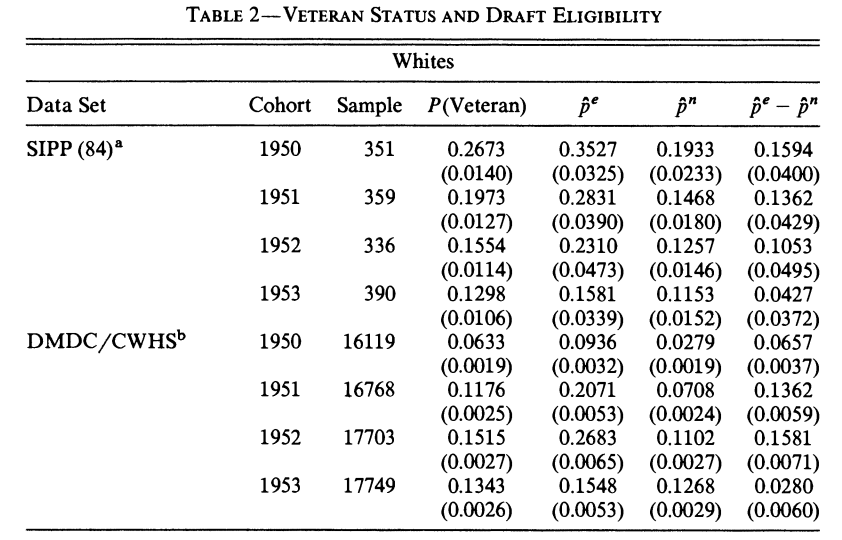
\includegraphics[width = 0.7 \linewidth]{angrist-first-stage}
\end{frame}


\begin{frame}
	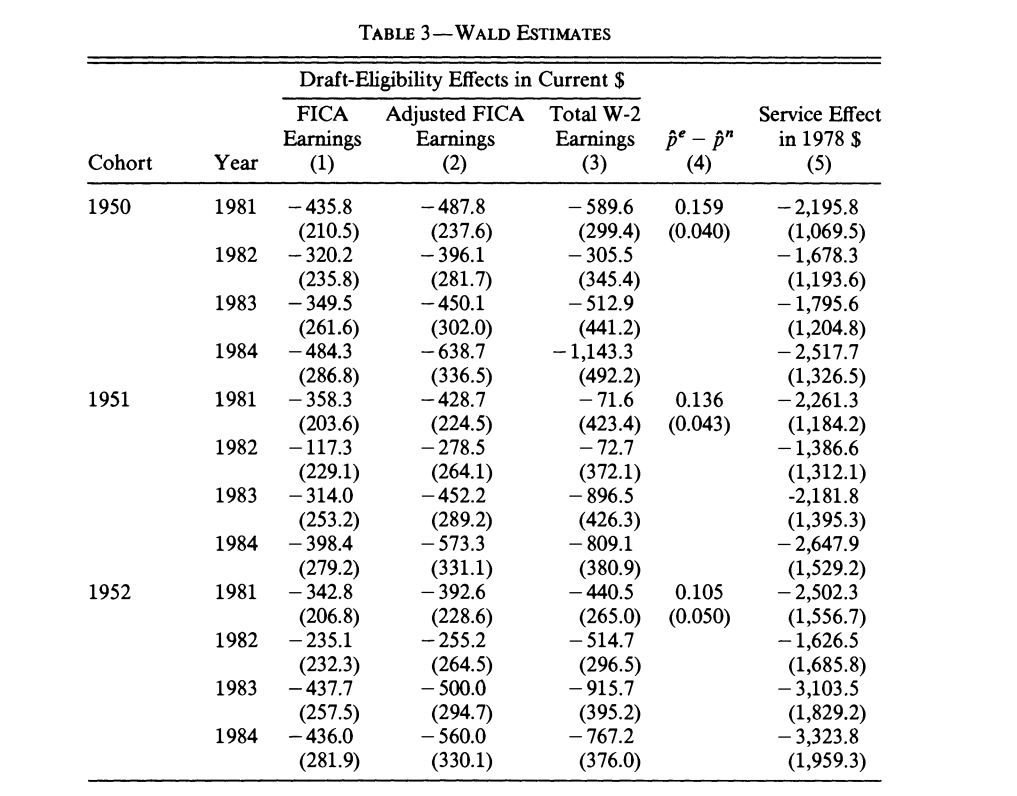
\includegraphics[width = 0.9 \linewidth]{angrist-wald}
\end{frame}


\begin{frame}{Visualizing LATE in this example}
	
	See diagrams \href{https://www.dropbox.com/s/nddh9vb6pjxvlng/2sls\%20diagrams.pdf?dl=0}{\underline{here}}
\end{frame}

%
%{	\begin{landscape}
%	\setbeamercolor{background canvas}{bg=}
%	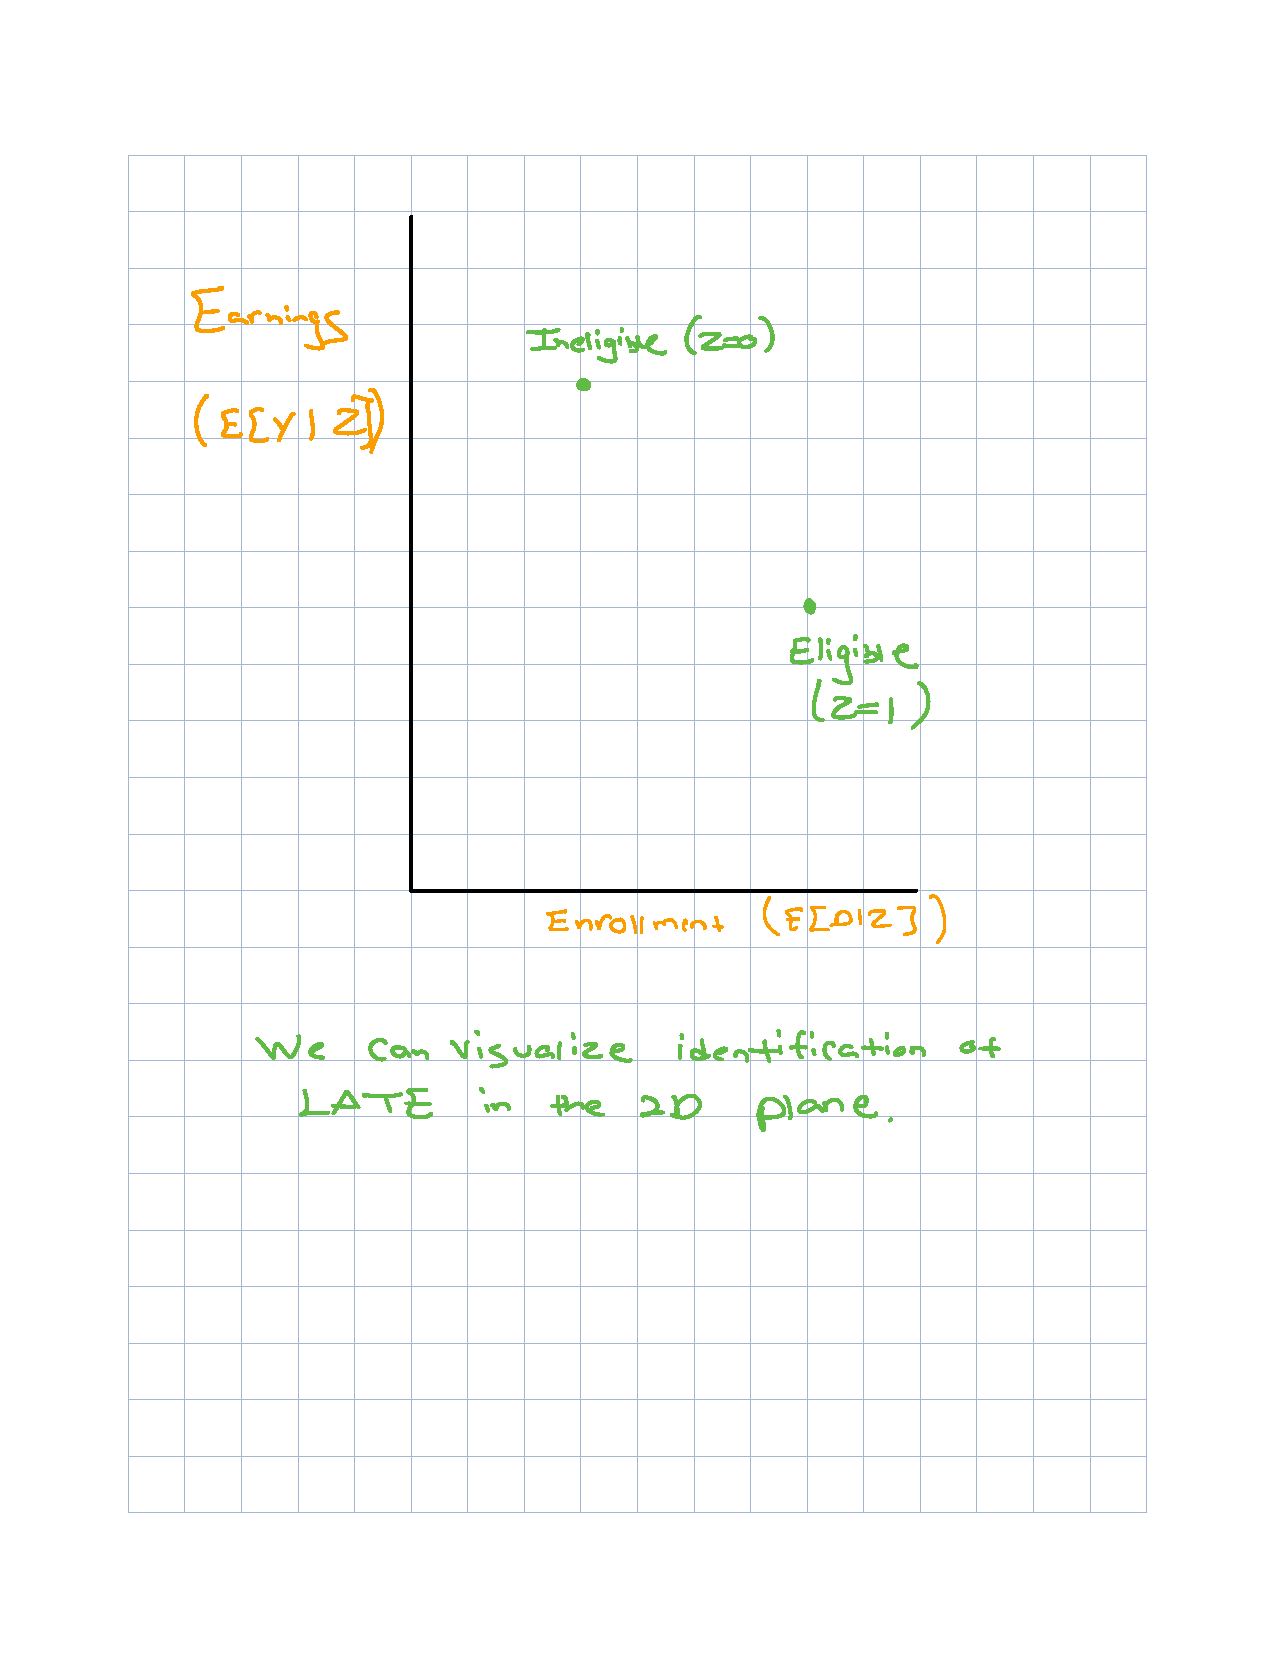
\includepdf{2sls diagrams.pdf}
%	\end{landscape}
%
%}




\begin{frame}
	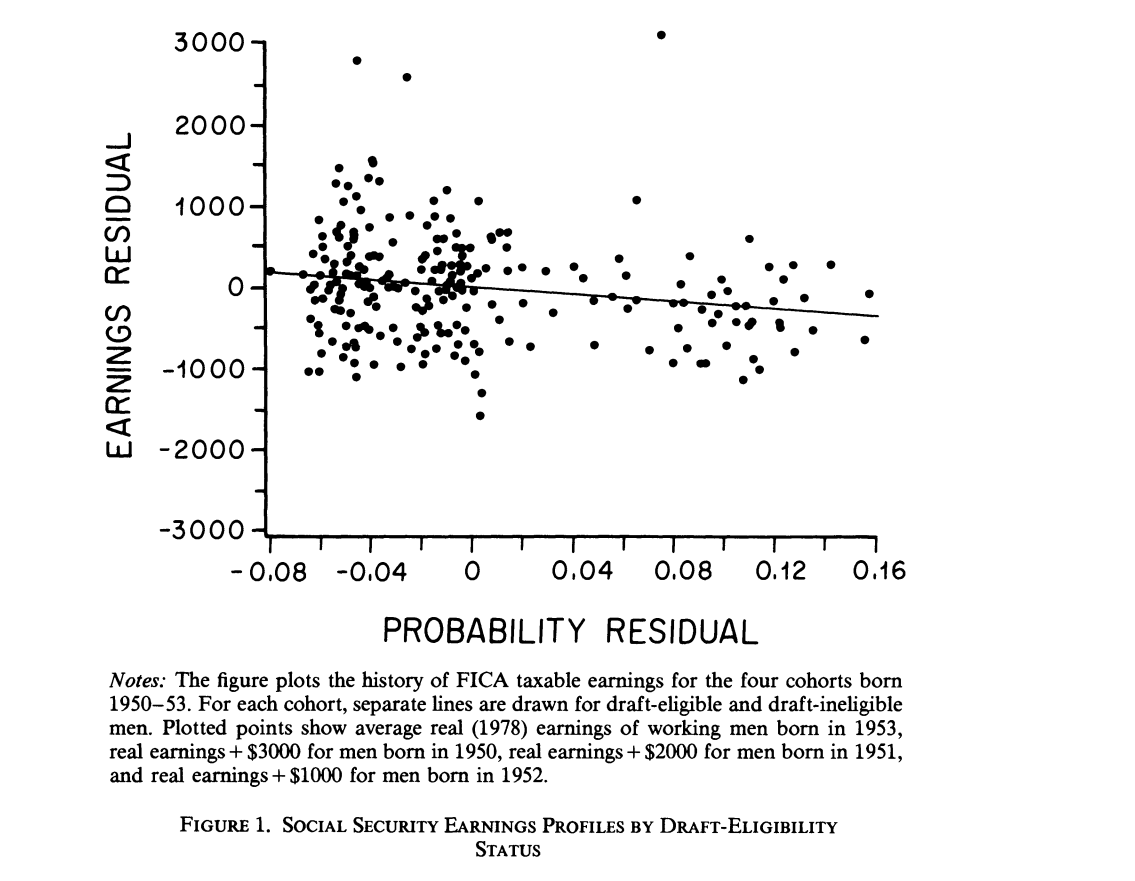
\includegraphics[width =0.9 \linewidth]{angrist-plot}
\end{frame}

\begin{frame}{Formalizing 2SLS with Multiple Instruments}
	\begin{wideitemize}
		\item
		We can formalize this procedure with what's called two-stage least squares with multiple instruments. 
		
		\item
		Suppose we have a vector of instruments $\bm{Z}_i$ (e.g. $Z_1$ is birthday 1, $Z_2$ is birthday 2)

\end{wideitemize}
\end{frame}

\begin{frame}{2SLS with multiple instruments}
\begin{wideitemize}
		\item
		Step 1 (first stage): Estimate $E[D_i | \bm{Z}_i]$ by estimating the OLS regression specification:
		
		$$D_i = \gamma_0 + \bm{Z}_i' \bm{\gamma}_1 + u _i$$
		
		E.g., estimate mean enrollment for each birthday			
		\pause
		\item
		Step 2: Construct the estimate of $E[D_i | Z_i]$ for each unit $i$:
		
		$$\hat{D}_i = \hat\gamma_0 + \bm{Z_i}' \bm{\hat\gamma}_1$$
		
		E.g., $\hat{D}_i$ is average enrollment for people with $i$'s birthday
		
		\pause
		\item
		Step 3 (second stage): use OLS to regress $Y_i$ on $\hat{D}_i$:
		
		$$Y_i = \beta_0 + \hat{D}_i \beta_1 + \epsilon_{i}$$
		
		E.g., regress earnings on average enrollment per birthday
		
		
		\pause
		\item
		$\hat\beta_1$ is our estimate of the (weighted) LATE
	\end{wideitemize}


\end{frame}


\begin{frame}
	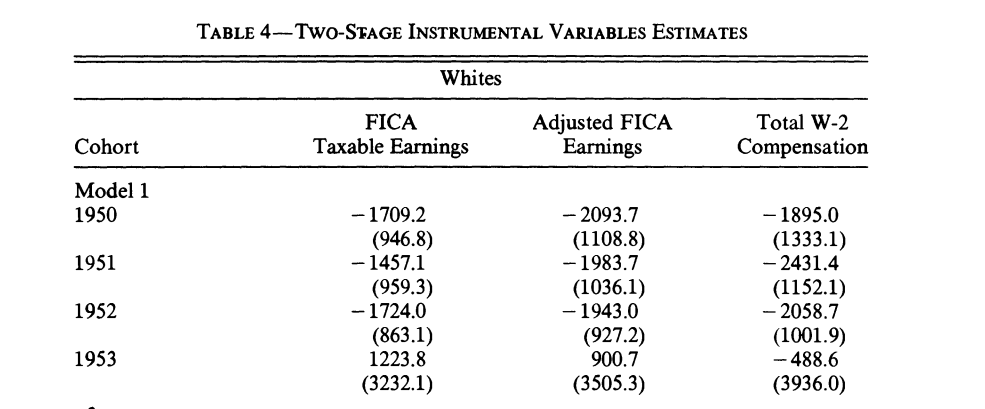
\includegraphics[width = 0.9 \linewidth]{angrist-2sls}
\end{frame}


\begin{frame}{Inference for 2SLS}
	\begin{wideitemize}
		\item
		How do we get standard errors for two-stage least squares estimates? 
		
		\pause
		\item
		We just showed that two-stage least squares is equivalent to running OLS with the regressor $\hat{D}$ from the first-stage? 
		
		\pause
		\item
		You might be tempted to just run this second stage regression and use the OLS standard errors. \pause{} But this will not give you the correct answer because it won't account for estimation error in $\hat{D}$
		
		\pause
		\item
		Luckily, it is easy to get correct 2SLS standard errors from Stata or other software packages
			\begin{itemize}
				\item
				\texttt{ivreg y (d=z) x, r} in Stata estimates 2SLS for treatment $d$ with instrument $z$ and controls $x$
			\end{itemize}
		
		\pause
		\item
		Where do these standard errors come from? 
	\end{wideitemize}
\end{frame}


\begin{frame}{Normality of reduced form and first stage}
	\begin{wideitemize}
		\item
		Remember that with a single instrument, $\hat\beta_{IV} = \hat\gamma_1 / \hat\pi_1$, where $\hat\gamma_1,\hat\pi_1$ are OLS estimates of
		\begin{align*}
			&Y_{i} = \gamma_0 +   Z_i \gamma_1 + \epsilon_{i} \\
			&D_i = \pi_0 + Z_i \pi_1 + u_i
		\end{align*}
	
		\pause
		\item
		We've shown that OLS estimates are asymptotically normally distributed (and these convergences hold jointly), so we will have
		
		$$\sqrt{N}\left( \left( \begin{array}{ll} \hat\gamma_1 \\ \hat\pi_1 \end{array} \right)- \left( \begin{array}{ll} \gamma_1 \\ \pi_1 \end{array} \right) \right) \rightarrow_d \mathrm{N}(0,\Sigma)$$
	
		\pause
		\item
		Can we learn from this the asymptotic distribution of $\hat\gamma_1 / \hat\pi_1$?
	\end{wideitemize}
\end{frame}

\begin{frame}{Delta method}
	\begin{wideitemize}
	\item
	Let $g(\hat\gamma_1, \hat\pi_1) = \hat\gamma_1 / \hat\pi_1$. \pause{} For $(\hat\gamma_1, \hat\pi_1) \approx (\gamma_1, \pi_1)$ a first-order Taylor expansion tells us that 
	$$g(\hat\gamma_1, \hat\pi_1) \approx g(\gamma_1,\pi_1) + \nabla g(\gamma_1,\pi_1) (\hat\gamma_1 - \gamma_1, \hat\pi_1 - \pi_1)' $$
	
	\noindent where $\nabla g(\gamma_1,\pi_1)$ is the gradient of $g$ evaluated at $(\gamma_1, \pi_1)$. 
	
	\item
	This implies that
	
	$$\sqrt{N}\left( \underbrace{ \frac{\hat\gamma_1}{\hat\pi_1}}_{g(\hat\gamma_1 , \hat\pi_1)} -  \underbrace{\frac{\gamma_1}{\pi_1} }_{g(\gamma_1,\pi_1)} \right) \approx  \nabla g(\gamma_1, \pi_1)\sqrt{N}\left( \left( \begin{array}{ll} \hat\gamma_1 \\ \hat\pi_1 \end{array} \right)- \left( \begin{array}{ll} \gamma_1 \\ \pi_1 \end{array} \right) \right)  $$
	
	\pause
	\item
	By the continuous mapping theorem, this converges in distribution to $\mathrm{N}(0,  \nabla g(\gamma_1, \pi_1) \Sigma  \nabla g(\gamma_1, \pi_1)')$.
	
	\pause
	\item
	We can estimate the variance with sample analogs (e.g. $\nabla g(\hat\gamma_1, \hat\pi_1))$).
\end{wideitemize}
\end{frame}

\begin{frame}{Weak identification}
	\begin{wideitemize}
		\item
		Note that $\hat\beta_{IV} = \hat\gamma_1 / \hat\pi_1$ is only well-defined for $\hat\pi_1 \neq 0$.
		
		\item
		As $\hat\pi_1 \rightarrow 0$, $|\hat\beta_{IV}| \rightarrow \infty$, so the IV estimator will be poorly behaved if $\hat\pi_1 \approx 0$.
		
		\pause
		\item
		This wasn't a problem in our asymptotics because we assumed $\pi_1 \neq 0$ (relevance), and as $N$ gets large, $\hat\pi_1 \rightarrow_p \pi_1$, so asymptotically $\hat\pi_1$ is near-zero with probability approaching zero. 
		
		\pause
		\item
		But in practice, $\hat\pi_1$ may sometimes be close to zero (relative to its standard error).
		
		\item
		In this case, the normal distribution above may provide a poor approximation to the distribution of $\hat\beta_{IV}$.  This is a problem known as \textit{weak identification}.
	\end{wideitemize}
\end{frame}


\begin{frame}{Weak Instruments - Monte Carlo}
Monte Carlo Simulation: No True Treatment Effect
$Y_i(d)= \eta + \nu; \hspace{1cm}  D_i = \pi_1 Z_i + \eta; \hspace{1cm}  \eta, \nu, Z_i \sim N(0,1)$ 	\\

\pause{}
Consider first a strong first-stage: $\pi_1 =1$ $\rightarrow$ $\frac{\pi_1}{SD(\pi_1)} \approx 22$

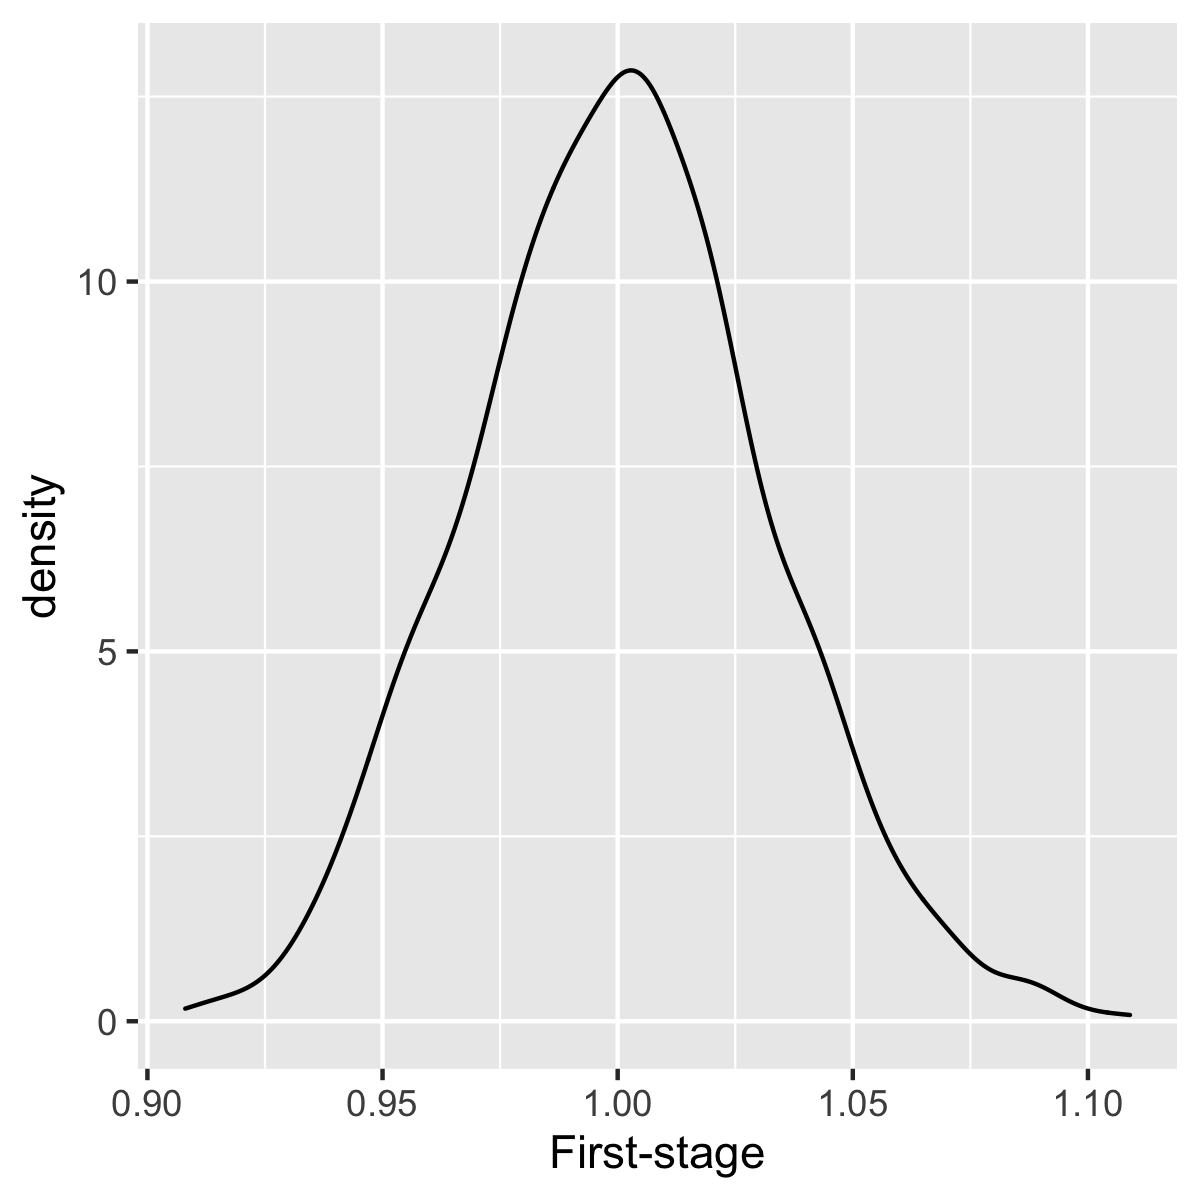
\includegraphics[width = 0.45 \linewidth]{fs-strong} \pause{} 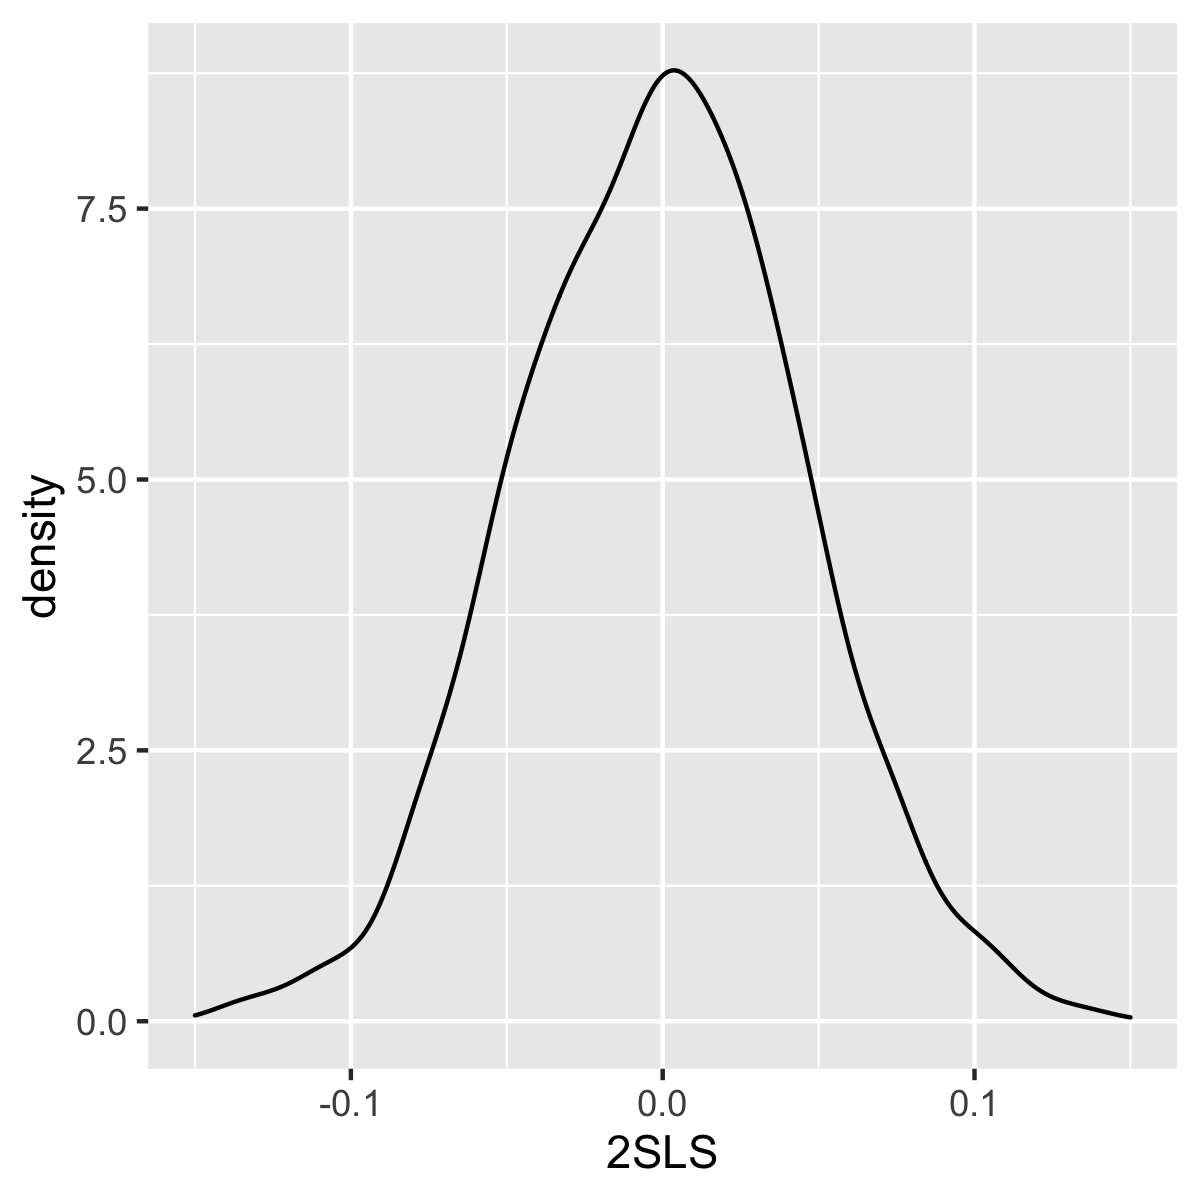
\includegraphics[width = 0.45 \linewidth]{iv-strong}
\end{frame}


\begin{frame}{Weak Instruments - Monte Carlo}
	Monte Carlo Simulation: No True Treatment Effect
	$Y_i(d)= \eta + \nu; \hspace{1cm}  D_i = \pi_1 Z_i + \eta; \hspace{1cm}  \eta, \nu, Z_i \sim N(0,1)$ 	\\
	
	Consider next a medium first-stage: $\pi_1 =0.25$ $\rightarrow$ $\frac{\pi_1}{SD(\pi_1)} \approx 7$
	
	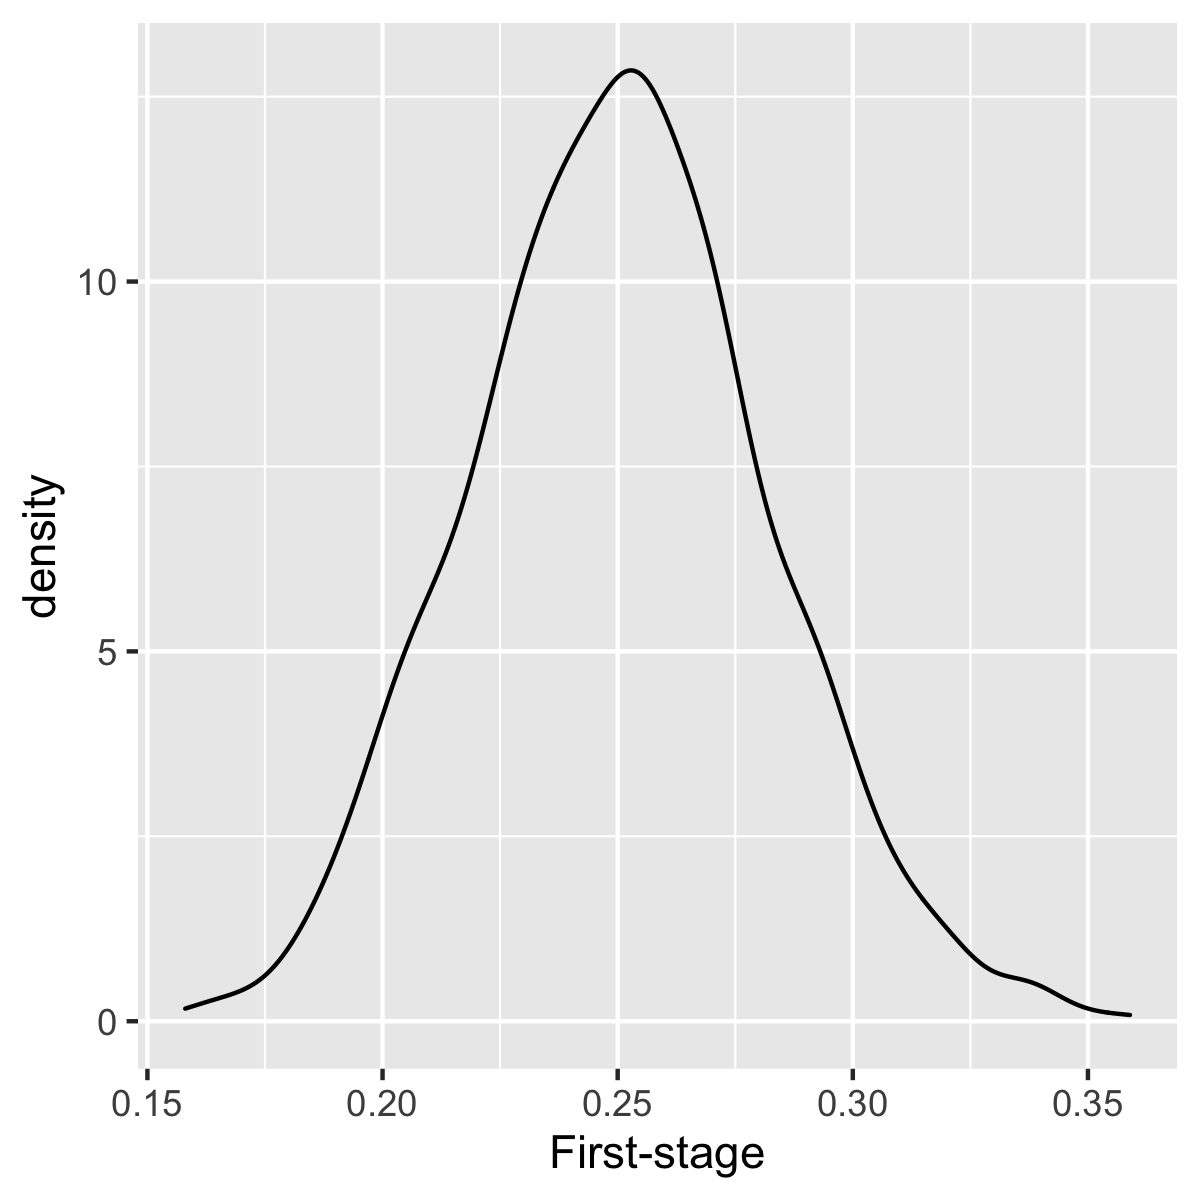
\includegraphics[width = 0.45 \linewidth]{fs-medium} \pause{} 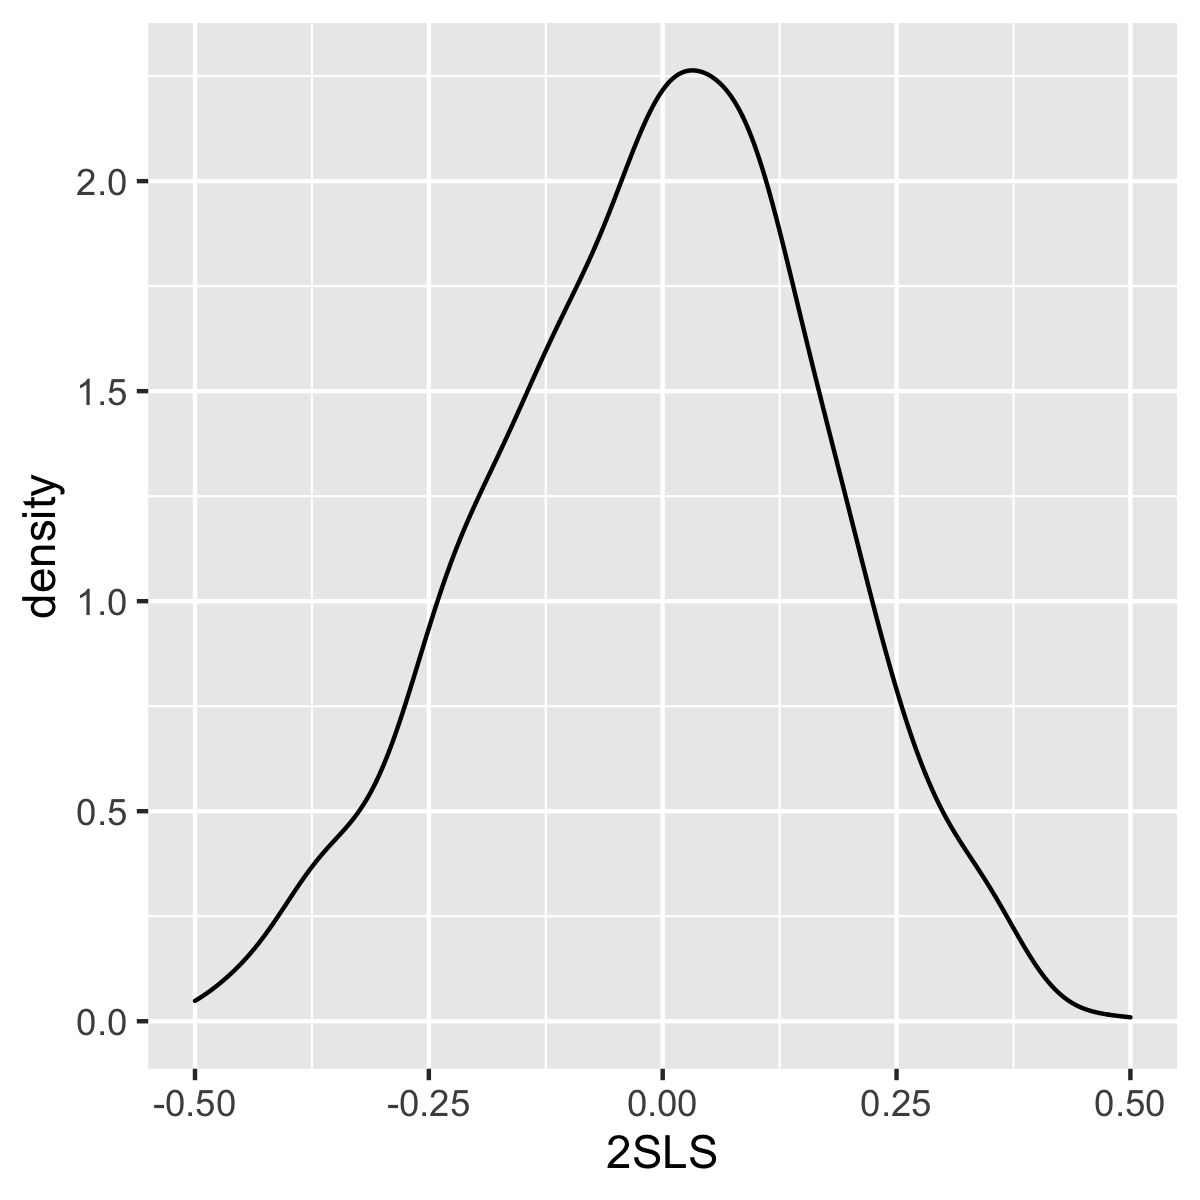
\includegraphics[width = 0.45 \linewidth]{iv-medium}
\end{frame}


\begin{frame}{Weak Instruments - Monte Carlo}
	Monte Carlo Simulation: No True Treatment Effect
	$Y_i(d)= \eta + \nu; \hspace{1cm}  D_i = \pi_1 Z_i + \eta; \hspace{1cm}  \eta, \nu, Z_i \sim N(0,1)$ 	\\
	
	Consider next a very weak first-stage: $\pi_1 =0.01$ $\rightarrow$ $\frac{\pi_1}{SD(\pi_1)} \approx 0.3$
	
	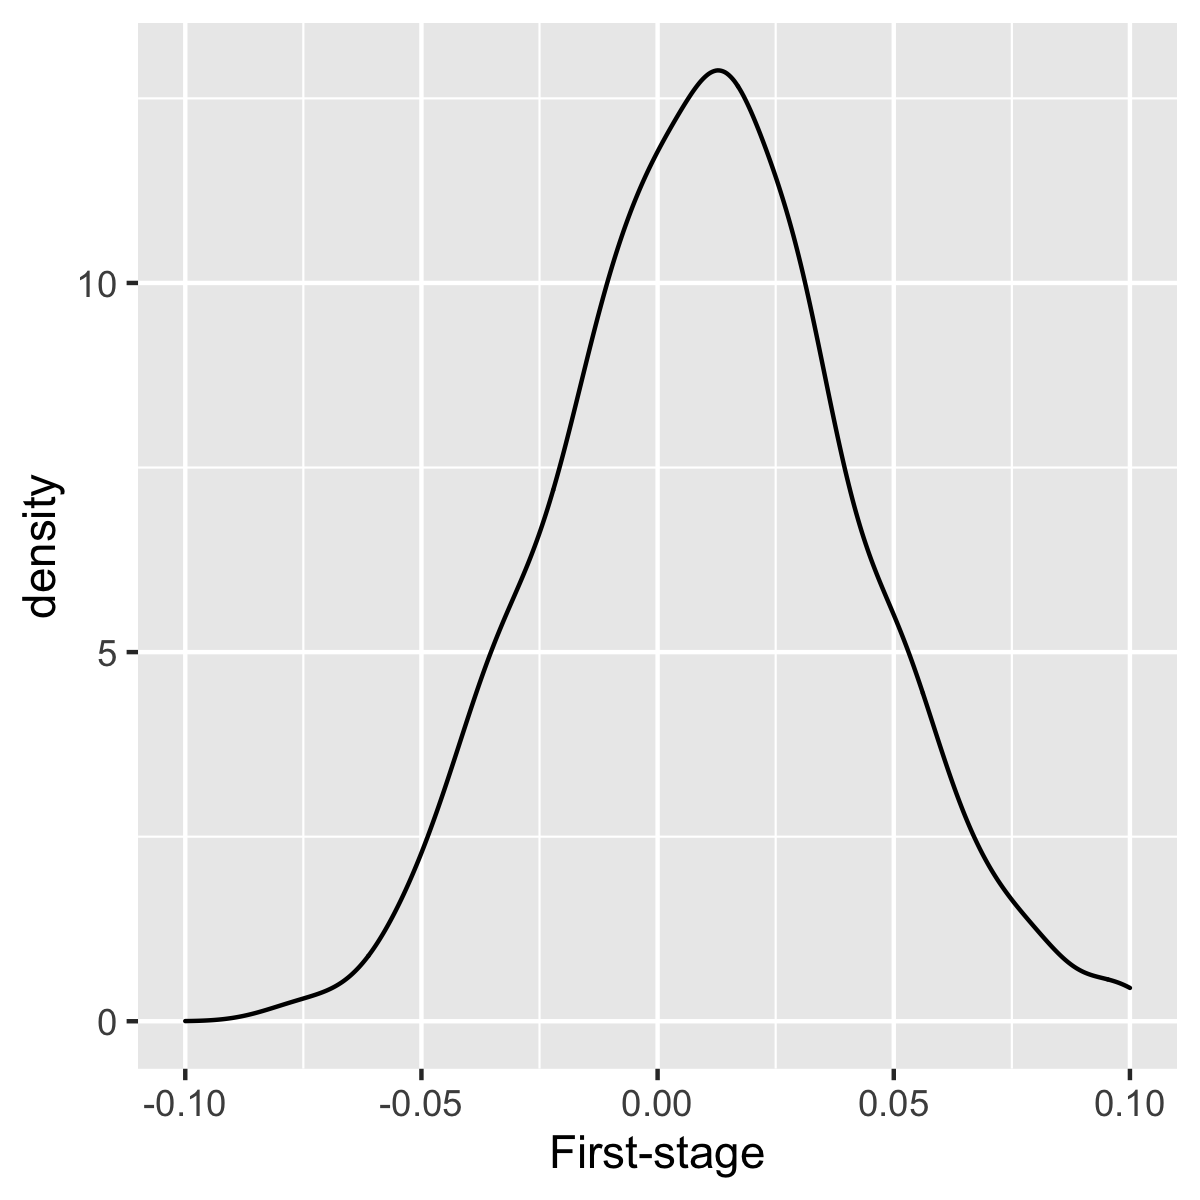
\includegraphics[width = 0.45 \linewidth]{fs-weak} \pause{} 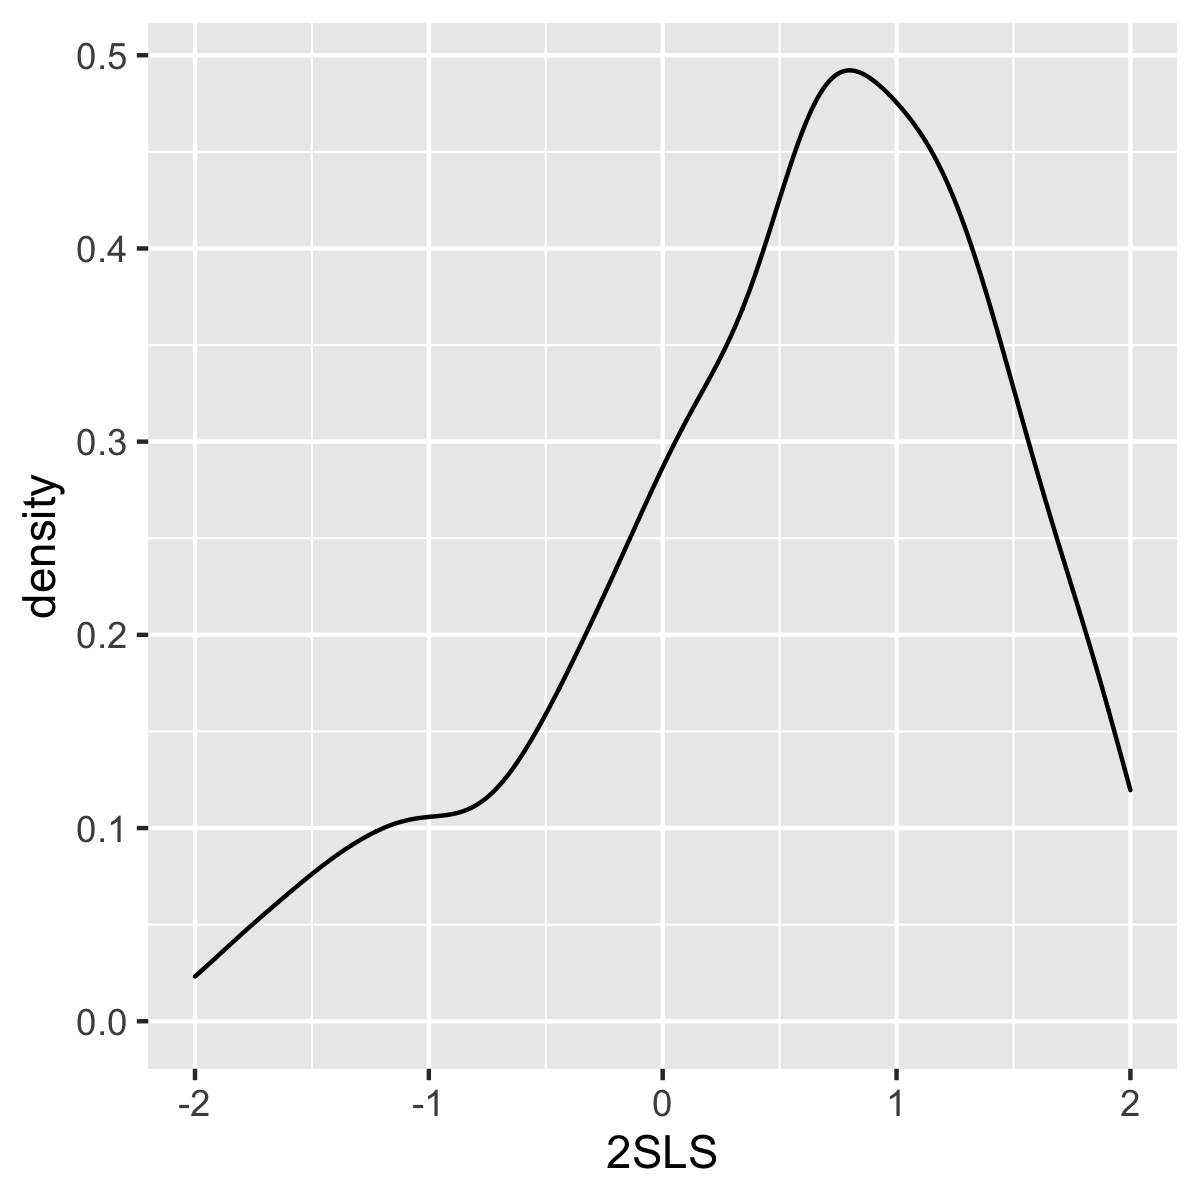
\includegraphics[width = 0.45 \linewidth]{iv-weak}
\end{frame}

\begin{frame}{Weak IV with multiple instruments}
	\vspace{0.2cm}
	A conceptually related problem arises when we have many instruments \pause{}
	
	\begin{itemize}
		\item Canonical example / cautionary tale: Angrist and Krueger (1991) interact the quarter-of-birth instruments with year and state of birth\pause{}
		\vspace{0.1cm}
		\item This decreased their SEs: better in-sample prediction of $D_i$\pause{}
		\vspace{0.1cm}
		\item Bound et al. (1995) famously show they get the same 2SLS estimates from randomly generated instruments
	\end{itemize}
	\pause{}
	\vspace{0.4cm}
	
	Intuition: when we have many instruments in the first-stage, we will ``overfit'' $D_i$. \pause{}
	
	
	\begin{itemize}
		\item  Imagine the extreme case, where every observation gets its own instrument (i.e. interact quarter-of-birth with individual)
		\item First-stage fit will be \emph{perfect}: $\hat{D}_i = \bm{\hat\pi_1}'Z_i =D_i$. So 2SLS = OLS numerically
		\item Thus the weak instrument problem arises from ``overfitting'' in the first stage
	\end{itemize}
	
\end{frame}


\begin{frame}{Testing for weak IV}
	\begin{wideitemize}
		\item
		A typical rule of thumb is to worry about weak instruments if the $F$-statistic on the instruments in the first stage is $<10$
		
		\item
		That is, run the first-stage regression
		
		$$D_i = \pi_0 + \bm{Z}_i ' \bm{\pi}_1 + \bm{X}_i' \bm{\pi}_2 + u_i$$
		
		\noindent and construct the $F$-statistic for the null $H_0: \bm{\pi}_1 = 0$. 
		
		\item
		With one instrument, the $F$-statistic is just the $t$-statistic on the instrument squared, so $F>10$ corresponds with $|t| > 3.2$.
		
		
	\end{wideitemize}
\end{frame}


\begin{frame}
	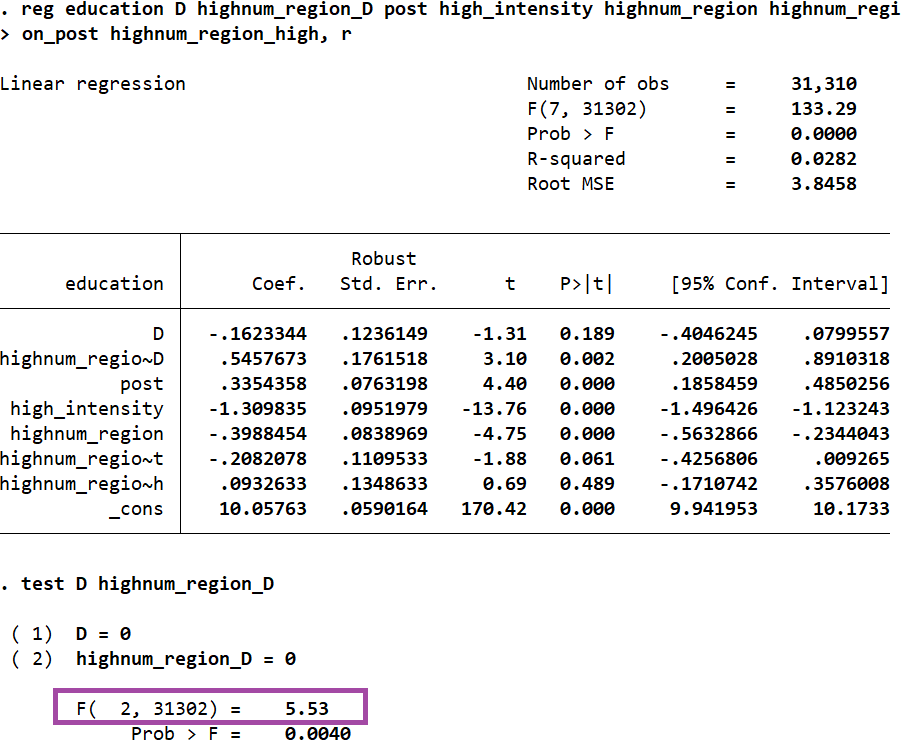
\includegraphics[width= 0.75\linewidth]{duflo_fs1.png}\\
	Here, the instruments are D and highnumregion\_D (confusing labels - sorry!). First-stage $F$ is 5.53
\end{frame}

\begin{frame}
	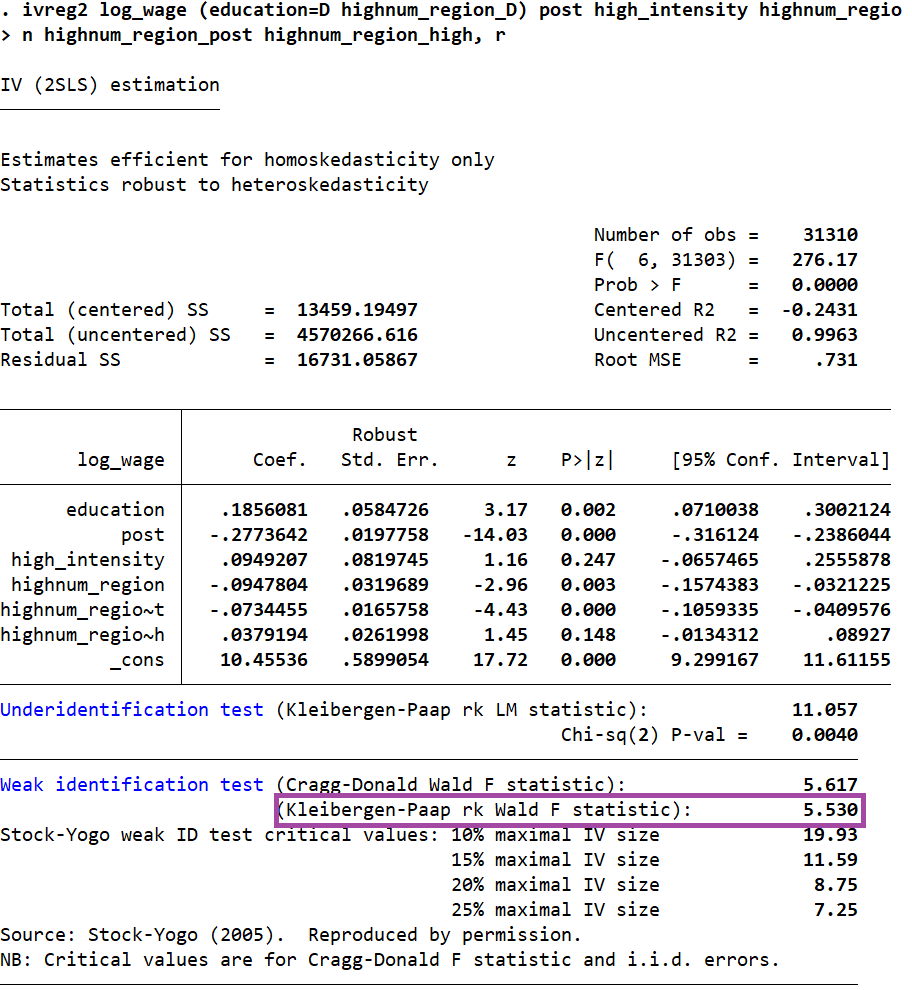
\includegraphics[width= 0.5\linewidth]{duflo_fs2.png}\\
	We can get the same $F$-stat directly from the ivreg2 command
\end{frame}

\begin{frame}{What do about weak instruments?}
	\begin{wideitemize}
		\item
		There are some ways to reducing over-fitting in the first-stage by splitting the sample (split sample or jacknife IV)
		
		\item
		There are alo some better ways to get confidence intervals when you have weak instruments
			\begin{itemize}
				\item 
				Most common is what are called Anderson-Rubin confidence sets (we won't have time to cover)
			\end{itemize}
		
		\item
		Can also try to increase the strength of the instrument by:
		
			\begin{wideitemize}
				\item
				Getting a larger sample
				
				\item
				Adding control variables that correlate with $D$ (but not strongly with $Z$)
				
				\item
				Thinking of a new instrument ;-)
			\end{wideitemize}
	\end{wideitemize}
\end{frame}
%% Evaluate the assumptions


%% Independence --- some violations for tax purposes

%% Exclusion --- hockey players

%% Relevance -- we've shown

%%Monotonicity --- probably okay


%% Add sectiosn on inference, weak IV, 

%% Add section about multiple instruments? 

%%
\end{document}


